\documentclass[utf8]{frontiersSCNS} % for Science, Engineering and Humanities and Social Sciences articles
%\documentclass[utf8]{frontiersHLTH} % for Health articles
%\documentclass[utf8]{frontiersFPHY} % for Physics and Applied Mathematics and Statistics articles

%\setcitestyle{square} % for Physics and Applied Mathematics and Statistics articles
\usepackage{url,hyperref,lineno,microtype,subcaption}
\usepackage{ulem}
\usepackage[onehalfspacing]{setspace}
\graphicspath{ {./plots/} }

% \linenumbers

% Leave a blank line between paragraphs instead of using \\

\def\keyFont{\fontsize{8}{11}\helveticabold }
\def\firstAuthorLast{Ozturk {et~al.}} %use et al only if is more than 1 author
\def\Authors{Abdurrahman Ozturk\,$^{1}$, Merve Gencturk\,$^{1}$, Karim Ahmed\,$^{1,2,*}$}
% Affiliations should be keyed to the author's name with superscript numbers and be listed as follows: Laboratory, Institute, Department, Organization, City, State abbreviation (USA, Canada, Australia), and Country (without detailed address information such as city zip codes or street names).
% If one of the authors has a change of address, list the new address below the correspondence details using a superscript symbol and use the same symbol to indicate the author in the author list.
\def\Address{$^{1}$Department of Nuclear Engineering, Texas A\&M University, USA\\$^{2}$Department of Materials Science and Engineering, Texas A\&M University, USA}
% The Corresponding Author should be marked with an asterisk
% Provide the exact contact address (this time including street name and city zip code) and email of the corresponding author
\def\corrAuthor{Karim Ahmed}
\def\corrEmail{karim.ahmed@tamu.edu}

\begin{document}
\onecolumn
\firstpage{1}

\title[]{Surface and Size Effects on the behaviors of point defects in irradiated crystalline solids} 

\author[\firstAuthorLast ]{\Authors} %This field will be automatically populated
\address{} %This field will be automatically populated
\correspondance{} %This field will be automatically populated

\extraAuth{}% If there are more than 1 corresponding author, comment this line and uncomment the next one.
%\extraAuth{corresponding Author2 \\ Laboratory X2, Institute X2, Department X2, Organization X2, Street X2, City X2 , State XX2 (only USA, Canada and Australia), Zip Code2, X2 Country X2, email2@uni2.edu}

\maketitle

\begin{abstract}

%%% Leave the Abstract empty if your article does not require one, please see the Summary Table for full details.
\section{}

We present an elaborate study of the surface and size effects on the transient and steady-state behaviors of point defects in irradiated solids. In this investigation, both pure Ni and binary Ni-Cr were utilized as model systems. We utilize the spatially-resolved rate-theory (SRRT) modeling approach, and directly account for the effects of dose rate, production bias, and defects recombination, reactions with volumetric sinks, and diffusion to surface sinks. Several simulations were conducted to investigate the effects of these parameters in both coupled and decoupled manners. In the presence of production bias, the effects of surface and size persist even as the surface to volume ratio decreases. This was associated with a surface-induced and size-regulated instability. This instability is only triggered above a critical size between 100-500 $nm$. The critical size decreases with increasing dose rate, increasing production bias, or lowering the temperature. Moreover, this instability results in a pattern that favors the separation of vacancies and interstitials. Once this pattern develops, anomalies in the dependence on size for the transient and steady-state concatenations of point defects and the surface/boundary sink strength are observed. These anomalies tend to render irradiation damage more sever. For pure Ni, it was shown that vacancy supersaturation increases with size, and the rate of increase also rises with size. For the binary Ni-Cr system, it was shown that the magnitude of enrichment/depletion of Ni/Cr at the boundary increases with size, and the width of the enrichment/depletion layer also increases with size. The results obtained here agree well with experimental observations in irradiated materials such as the formation of void denuded zones adjacent to grain boundaries and the size and temperature dependence of the radiation resistance of nanomaterials. The size-dependent behaviors reported here also shed new light on the radiation tolerance of nanomaterials, i.e., the irradiation-induced instabilities are suppressed in such materials. Lastly, the implications of the results obtained here on the development of efficient reduced order models or the utilization of ion irradiation as a surrogate to neutron irradiation are discussed.

\tiny
 \keyFont{ \section{Keywords:} point defect equations, rate theory, proton irradiation, neutron irradiation, electron irradiation, radiation damage, radiation-induced segregation, MOOSE} %All article types: you may provide up to 8 keywords; at least 5 are mandatory.
\end{abstract}

\clearpage
\section{Introduction}

Nuclear energy is an important source for the production of emission-free electricity. It has the highest power density and reliability among all forms of energy. Several new reactor designs are being developed to render nuclear energy more efficient, safe, and economic. The main limitation in deploying these novel designs is the qualification of novel materials capable of serving in such harsh environments.

Reactor materials operate under extreme conditions of irradiation, high temperature, high stress, and corrosive media. In such environments, these materials experience microstructural changes that result in the degradation of their physical, mechanical, and thermal properties. Some of the main consequences of microstructural changes are radiation embrittlement, irradiation creep, irradiation growth, void swelling, and high temperature helium embrittlement. Irradiation effects on materials need to be understood to predict their performance and hence facilitate the advancement of nuclear energy applications \citep{Vanderlaan2012,English2003,ryabikovskaya2021,yingling2021}.

Understanding irradiation effects on in-reactor materials is very challenging. First, it is very expensive to run in-reactor experiments. Second, the handling of the resultant radioactive material demands special treatment and equipment. Third, the relatively low dose rate experienced in normal operation requires performing long term experiments that might need to run for years to collect critical data. Fourth, it is extremely difficult to set up reactor experiments to simulate the materials response to transient and abnormal conditions such as in accidents. Fifth, it is also a cumbersome task to separate the combined effects of irradiation, temperature, and stress in such experiments. Lastly, the data obtained from the experiments carried out in a specific reactor might be irrelevant to new reactor designs with different operating conditions.

Two main approaches are currently in use to overcome these difficulties. In the first approach, ion irradiation is utilized to mimic neutron irradiation. Ion irradiation experiments can be conducted in ion-beam laboratories and using accelerators. Moreover, because of their high dose rate, accelerated irradiation experiments can be performed in a matter of hours or days \citep{shao2017, sun2017, krasheninnikov2010, was2014, zhang2018}. Nonetheless, because of this large difference in dose rate, the extrapolation of the ion irradiation data to assess the behavior of materials under neutron irradiation is questionable. The second approach leverages the modern computational tools to implement physics-based and data-driven models to simulate the response of materials to neutron irradiation. Nonetheless, because of the inherently multiscale nature of the problem, conducting high fidelity simulations is still unfeasible. 

While the two approaches currently have their limitations, they have demonstrated several successes in elucidating irradiation effects on materials. \citep{was_emulation_2002} examined 304SS and 316SS cladding steels samples to evaluate whether proton irradiation can be utilized to simulate neutron irradiation. They irradiated the samples with neutrons at 548 $K$ and protons at 633 $K$ to offset the difference in dose rate. As a result of their investigations, it was shown that radiation-induced segregation (RIS) behavior at the grain boundary and the defect kinetics under neutron irradiation can be replicated using proton irradiation \citep{was_emulation_2002}. Nonetheless, large discrepancies between ion and neutron irradiation are also reported in other situations \citep{was2017}.  For the second approach, a divide and conquer strategy is often employed to decouple the distinct irradiation-induced phenomena that usually span multiple length and time scales. Moreover, different atomistic, mesoscale, and macroscale models are often utilized to relate the evolution of the atomistic- and micro-structure of irradiated materials to the resultant change of their properties \citep{was2017}. Nevertheless, the decoupled models proved to be still difficult to solve because of their multiphysics nature. 

The computational approach is, however, very promising given the ever-increasing computational power. Moreover, it can be used to either guide the ion irradiation experiments to better simulate neutron irradiation or extrapolate their results to neutron irradiation \citep{xu2012}. Classically, several approximations were utilized to lower the computational cost associated with numerical simulations. For instance, in rate-theory models that simulate long term irradiation effects, a homogenization scheme is often utilized, which ignores the underlying microstructure and spatial resolution of irradiation defects \citep{was2017}. Clearly, this limits the model to obtain predictions only about the averages of quantities of interest. However, other models that relax these assumptions were introduced based on the so-called spatially resolved rate-theory (SRRT), which requires solving coupled partial differential equations representing different types of defects \citep{bennett1975, warburton1975, franklin1975, thompson1974, ullmaier1980}. Several recent investigations have implemented these models to gain more insight on irradiation effects on materials. \citep{short2016} solved rate theory equation by accounting for injected interstitials and investigated the changes in the spatial void swelling profiles. \citep{chen2019} studied proton irradiation induced dislocation loops in modified 310S steels. They used a series of rate equations for different defect types including self-interstitial atoms (SIAs), vacancies, interstitial clusters, vacancy clusters, dislocation lines and grain boundaries. \citep{choi2020} used rate theory to understand irradiation creep behavior of iron-based alloys exposed to stress-applied environment. They coupled rate theory equations with a model for creep and analyzed the behavior at different dose rates. \citep{saidi2021} presented an approach to study the effect of dose rate on radiation damage accumulation in polycrystalline systems in the presence of internal and grain boundary sink strengths. They used both proton and electron irradiation in their study and calculated the relation between internal sink strength to the grain boundary sink strength. All these studies demonstrated the importance of resolving the spatial dependences of both the underlying microstructure and irradiation defects for developing better understanding of the behavior of materials under irradiation.

Here, we follow the SRRT approach to investigate the surface and size effects on the transient and steady-state kinetics of point defects in irradiated solids. Moreover, we take into consideration the effects of dose rate, production bias, and defects recombination, reactions with distributed/volumetric sinks, and diffusion to localized/surface sinks. While there are a few attempts in literature to study the surface and size effects (\citep{yang2010,demkowicz2011,xu2012}), they are limited to small sizes and ignored one or more of the main irradiation conditions or defect mechanisms accounted for here. Indeed, this work demonstrates the importance of considering the combined effects of surface, size, dose rate, production bias, and temperature on the response of materials to irradiation. Specifically, we show that a few transient and steady-state irradiation-induced instabilities could be observed only if all these factors were accounted for simultaneously in the simulations. Furthermore, these instabilities lead to the development of different patterns in the steady-state concentrations of point defects that can either increase or decrease their ability to cluster into extended defects, and hence determine the extent of irradiation damage in materials.

This paper is organized as follows. In section 2, the SRRT approach is outlined and its numerical implementation is detailed. In section 3, the results are presented and discussed. Lastly, in section 4, concluding remarks are drawn and recommendations for future studies are given.

% For Original Research Articles \citep{conference}, Clinical Trial Articles \citep{article}, and Technology Reports \citep{patent}, the introduction should be succinct, with no subheadings \citep{book}. For Case Reports the Introduction should include symptoms at presentation \citep{chapter}, physical exams and lab results \citep{dataset}.

\newpage
\section{Methodology}

% For requirements for a specific article type please refer to the Article Types on any Frontiers journal page. Please also refer to  \href{http://home.frontiersin.org/about/author-guidelines#Sections}{Author Guidelines} for further information on how to organize your manuscript in the required sections or their equivalents for your field

% For Original Research articles, please note that the Material and Methods section can be placed in any of the following ways: before Results, before Discussion or after Discussion.

\subsection{Balance Equations for Point Defects}
 The concentration of single vacancies and interstitials (e.g., point defects), $C$, are described mathematically by the chemical rate balance equations given in following sets of equations,

\begin{equation}
  \begin{aligned}
    &\frac{\partial C_i}{\partial t} = K_0 - K_{iv}C_iC_v - K_{is}C_iC_s + \nabla\cdot D_i\nabla C_i\\
    &\frac{\partial C_v}{\partial t} = (1+b)K_0 - K_{iv}C_iC_v - K_{vs}C_vC_s + \nabla\cdot D_v\nabla C_v
  \end{aligned}
  \label{equation:point_defect_equations}
\end{equation}

    There are different terms with different rate coefficients as seen in Eq. \ref{equation:point_defect_equations}. The first term on the RHS is a source term, representing defect generation with rate constant of \textit{K\textsubscript{0}}. Defect production can be either uniform or non-uniform depending on irradiation type. The second term is a reaction term, referring to the recombination process between the defect \textit{x} and the defect \textit{y} with a rate constant of \textit{K\textsubscript{xy}}. The third term is also a reaction term, representing the reaction between the defect \textit{x} and the sink \textit{s} with a rate constant of \textit{K\textsubscript{xs}}.
    \begin{equation}
        \begin{aligned}
            &K_{xy} = 4\pi r_{xy}(D_x+D_y) \\
            &K_{xs} = 4\pi r_{xs}D_x \\
        \end{aligned}
        \label{equation:rate_constants}
    \end{equation}
    where $r_{xy}$ and $r_{xs}$ are interaction radii for the reaction of defect \textit{x} with defect \textit{y} or a sink \textit{s}. Interaction radii are usually taken as a multiple of the lattice constant,a, e.g., 10a. 
    
    In this study, the sink concentration is assumed constant and uniformly distributed over domain. The last term represents the  diffusion of defects \citep{motta2017,was2017}. Lastly, b is a production bias factor to be discussed next.
    
    In principle, atomic collisions create vacancy-interstitial pairs (Frenkel Pairs), and they might recombine to restore the equilibrium state. Nonetheless, irradiation cascades usually have an underlying structure with vacancy rich core and interstitial rich periphery. This leads to the formation of small vacancy and interstitial clusters. Interstitial clusters are usually more thermally stable than their vacancy counterparts, which usually dissolve and inject vacancies back to the matrix. Eventually, this results in the presence of more single vacancies surviving the cascade stage than single interstitials. Moreover, the presence of dislocations in materials before irradiation (because of processing) may also increase this imbalance in point defects because of the preferential absorption of dislocations to interstitials. For models that are concerned with the long term irradiation effects, as in the case here, this defect imbalance is usually captured using a bias factor in the production rate \citep{motta2017,was2017}. We follow the same procedure here by introducing the bias factor, b, in the production rate of vacancies.
    
    Another common form for the point defect equations is usually written by using sink strength, \textit{k},  definition for the defect-sink reaction term as follows,

    \begin{equation}
      \begin{aligned}
        &k_i^2D_iC_i = K_{is}C_iC_s \\
        &k_v^2D_vC_v = K_{vs}C_vC_s \\
      \end{aligned}
      \label{equation:sink_reaction_term}
    \end{equation}\\
    Subsituting Eq. \ref{equation:sink_reaction_term} into Eq. \ref{equation:point_defect_equations} gives,
    \begin{equation}
      \begin{aligned}
        &\frac{\partial C_i}{\partial t} = K_0 - K_{iv}C_iC_v - k_i^2D_iC_i + \nabla\cdot D_i\nabla C_i\\
        &\frac{\partial C_v}{\partial t} = (1+b)K_0 - K_{iv}C_iC_v - k_v^2D_vC_v + \nabla\cdot D_v\nabla C_v\\
      \end{aligned}
      \label{equation:point_defect_equations_sink_strength}
    \end{equation}

    This definition of sink strength is beneficial in understanding the point defect-sink reactions. It is also important in evaluating the differences between the homogenized rate-theory and the spatially-resolved rate theory. We will utilize it here also to assess the  difference in the predictions between the two theories for different microstructures and irradiation conditions.\\

\subsection{Non-dimensionalization of Balance Equations for Point Defects}
    To simplify the implementation of the equations and improves the convergence, non-dimensionalization of the above equations was performed. Specifically, the following non-dimensionalization scheme and scaling factors are introduced.
    
    \begin{equation}
      \begin{aligned}
        &X = \Omega C\\
        &\tau = \frac{t}{\omega}\\
      \end{aligned}
      \label{equation:non-dimensionalization_variables}
    \end{equation}\\
    where ${\Omega}$ is the atomic volume in ${m^3}$, ${l}$ is a characteristic length scale in ${m}$, and ${\omega}$ is a characteristic time scale in ${s}$, ${\omega= l^2/D_i}$\\
    \\
    After substituting Eq. \ref{equation:non-dimensionalization_variables} into \ref{equation:point_defect_equations} and reorganizing, the final form  of the non-dimensionalized dynamical system becomes,
    
    \begin{equation}
      \begin{aligned}
        &\frac{\partial X_i}{\partial\tau} = \Omega\omega K_0 - \frac{\omega K_{iv}}{\Omega}X_iX_v - \frac{\omega K_{is}}{\Omega}X_iX_s + \omega D_i\nabla^2 X_i\\
        &\frac{\partial X_v}{\partial\tau} = (1+b)\Omega\omega K_0 - \frac{\omega K_{iv}}{\Omega}X_iX_v - \frac{\omega K_{vs}}{\Omega}X_vX_s + \omega D_v\nabla^2 X_v\\
      \end{aligned}
      \label{equation:non-dimensionalized_point_defect_equations}
    \end{equation}
    defining new non-dimensionalized parameters,\\
    \begin{equation}
      \begin{aligned}
        &\widetilde{K_0}=\Omega\omega K_0,
            &\widetilde{D_i}=\frac{D_i}{D_i}=1\\
        &\widetilde{K_{iv}}=\frac{\omega K_{iv}}{\Omega},
            &\widetilde{D_v}=\frac{D_v}{D_i}\\
        &\widetilde{K_{xs}}=\frac{\omega K_{xs}}{\Omega}, 
            &\widetilde{\nabla}=l^2\nabla\\
      \end{aligned}
      \label{equation:non-dimensionalized_parameters}
    \end{equation}
    the final form is,\\
    \begin{equation}
      \begin{aligned}
        &\frac{\partial X_i}{\partial\tau} = \widetilde{K_0} - \widetilde{K_{iv}}X_iX_v - \widetilde{K_{is}}X_iX_s + \widetilde{\nabla}^2 X_i\\
        &\frac{\partial X_v}{\partial\tau} = (1+b)\widetilde{K_0} - \widetilde{K_{iv}}X_iX_v - \widetilde{K_{vs}}X_vX_s + \widetilde{D_v}\widetilde{\nabla}^2 X_v\\
      \end{aligned}
      \label{equation:non-dimensionalized_point_defect_equations}
    \end{equation}
    The non-dimensionalized form of Eq. \ref{equation:point_defect_equations_sink_strength} can be derived easily from Eq. \ref{equation:non-dimensionalized_point_defect_equations} by using Eq. \ref{equation:sink_reaction_term}.
    \begin{equation}
      \begin{aligned}
        &\frac{\partial X_i}{\partial\tau} = \widetilde{K_0} - \widetilde{K_{iv}}X_iX_v - \widetilde{k_{i}^2}X_i + \widetilde{\nabla}^2 X_i\\
        &\frac{\partial X_v}{\partial\tau} = (1+b)\widetilde{K_0} - \widetilde{K_{iv}}X_iX_v - \widetilde{k_{v}^2}\widetilde{D_v}X_v + \widetilde{D_v}\widetilde{\nabla}^2 X_v\\
      \end{aligned}
      \label{equation:non-dimensionalized_point_defect_equations_sink_strength}
    \end{equation}
    non-dimensionalized sink strengths are,
    \begin{equation}
      \begin{aligned}
        &\widetilde{k_{x}^2}={l^2 k_{x}^2}
      \end{aligned}
      \label{equation:non-dimensionalized_parameters_sink_strength}
    \end{equation}\\
    
\subsection{Model Parameters and Numerical Implementation}

    The Multiphysics Object-Oriented Simulation Environment (MOOSE) is used as a tool to solve the balance equations for point defects numerically. MOOSE is an open-source framework that provides users with several capabilities to solve partial differential equations (PDEs). It contains a multitude of built-in features such as different linear and non-linear solvers, different integration schemes, mesh and time adaptivity, mesh generation and post-processing options, and many more. \citep{permann2020}. MOOSE has been utilized before to investigate irradiation effects and coevolution of microstructure and properties in materials \citep{ahmed2020,tonks2018,ahmed2018,ozturk2018,ozturk2019,abdoelatef2019,badry2019,badry2021}.
    
    %Equations were solved in both Cartesian and spherical coordinates to represent planar and spherical geometries, respectively.
    Simulations in this study are modeled in 1D domains. Equations were first solved for a test case in both Cartesian and spherical coordinates to represent planar and spherical geometries, respectively. The difference in results was not significant, so Cartesian coordinate system was used in simulations unless otherwise stated. The domain boundaries are assumed to represent free surfaces or grain boundaries. Hence, they are modeled as perfect and neutral, i.e., point defects take on their equilibrium values at the boundaries. Sinks such as voids and dislocations, which are present in the bulk, are assumed uniformly distributed with a concentration of 1e18 $m^{-3}$. 1D first-order Lagrange elements were used for spatial discretization and a second-order implicit scheme was utilized for time integration. A grid size in the range of 0.1-1 $nm$ was used in the simulations. Mesh sensitivity studies were conducted, and the results reported here are confirmed to be independent of grid size within the range mentioned. A length scale, l, that is much smaller than the lowest grain size was used in our simulations. Since the smallest grain size was 5nm, a length scale of 0.1 nm was used in all simulations.
    
    Ni-based alloys are used in many nuclear reactors because of their excellent corrosion resistance and high mechanical properties. For example, Ni-based alloys containing 15-30\% Cr are generally used in the cooling systems of reactors due to their corrosion resistance. Ni-Cr based alloys are also candidates for structural materials in molten-salt reactors. Therefore, here we selected Nickel as a base material for this study. Ni properties used in the simulations: lattice parameter, $a$, is 0.352 $nm$, atomic volume, $\Omega$ , is 0.01206 $nm^3$, migration energy for interstitial, $E_{m,i}$, is 0.30 $eV$ , migration energy for vacancy, $E_{m,v}$, is 1.30 $eV$ , formation energy for interstitial, $E_{f,i}$, is 4.27 $eV$ , formation energy for vacancy, $E_{f,v}$, is 1.60 $eV$ , pre-exponential diffusion coefficient for interstitial, $D_{0,i}$, is 1e-7 $m^2/s$, and pre-exponential diffusion coefficient for vacancy, $D_{0,v}$, is 6e-5 $m^2/s$ \citep{walgraef1996,zhao2016}. In most of the simulations presented here, a temperature of 773 $K$ was assumed unless otherwise explicitly stated. The temperature dependence of diffusion coefficients follows the well-known Arrhenius relationship. Reaction rate constants, $K_{iv}$, $K_{is}$ and $K_{vs}$ are calculated using Eq. \ref{equation:rate_constants}. The value for the interaction radii, $r_{xy}$, is 3.52 $nm$. The calculated reaction rate constants, $K_{xy}$ and $K_{xs}$, are 4.8958e-17 $m^3/s$ and 3.7795e-21 $m^3/s$.
    
% \textcolor{red}{
% Tables should be inserted at the end of the manuscript. Please build your table directly in LaTeX.Tables provided as jpeg/tiff files will not be accepted. Please note that very large tables (covering several pages) cannot be included in the final PDF for reasons of space. These tables will be published as \href{http://home.frontiersin.org/about/author-guidelines#SupplementaryMaterial}{Supplementary Material} on the online article page at the time of acceptance. The author will be notified during the typesetting of the final article if this is the case.
% }

\section{Results}
   
    The defect production term, $K_0$, depends on the type of the incident radiation. Its magnitude and spatial dependence are determined by the interactions of incoming particles with the target material. Neutrons have an energy spectrum that varies by a couple of orders of magnitude. Defect generation is possible at different energies for neutrons. Also, because of their charge neutrality, they are able to travel through materials to farther distances corresponding with their energies. Thus, they cause a uniform or flat-like defect production profile in target materials. Electron and protons are not able to penetrate as much as neutrons do, but for small domain sizes ($<$ 5 $\mu m$), their defect production can be assumed uniform as well. On the other hand, ions have a relatively narrow energy channel width, which is almost monoenergetic. They also cannot penetrate through material excessively because of their high electronic energy loss in collisions. This characteristic behavior of ions causes a non-uniform defect production profile. We have conducted simulations for both uniform and non-uniform irradiations. While there are several quantitative differences, the main qualitative trends of interest are similar. Therefore, here, for the sake of brevity and clarity, we will discuss only the results of uniform irradiation. With regards to the different rates, different point defects rates are expected for different irradiation types and temperatures. However, for investigations concerned with long term irradiation effects usually a simple range representing different types is employed. For instance, a range of 1e-4 to 1e-2 $dpa/s$ for energetic electrons/protons/ions and a range of 1e-8 to 1e-6 $dpa/s$ for neutrons are usually quoted \citep{was2017}.
    
    The defect production bias, $b$, also strongly depends on the type of irradiation. This because of the different cascade structures and densities produced by different types. Neutrons and heavy ions result in highly dense cascades, leading to high bias (because of the higher stability of small interstitial clusters relative to their vacancy counterparts). Electrons, on the other hand, result in isolated point defects, with very low bias. Protons and light ions lie between those two limits \citep{was2017}.

    In most rate-theory based studies, most of the focus is usually on the effects of temperature, dose rate, and sink densities. The effects of size and isolated/discrete surfaces are often ignored. Only a few studies \citep{yang2010,demkowicz2011} investigated to some extent these effects. However, those studies were limited to small size grains (e.g., nanograins) and ignored the effect of production bias. As will be evident from our study here, surface and size effects play a major role in determining both the transient and steady profiles of point defects in irradiated solids. Moreover, it will be demonstrated that there is a critical size at which a nonlinear instability is triggered, which in turn results in a specific pattern that favors the separation of vacancies and interstitials and hence promotes irradiation damage. That critical size is influenced by does rate, production bias, and temperature. Therefore, considering the influences of temperature, size, dose rate, production bias, and their combined effect is required in any future studies of irradiation effects and ignoring any of these principal parameters is unjustifiable.\\

\subsection{Surface and size effects on the transient and steady-state behaviors of point defects in irradiated Ni}

To validate the numerical implementation of the balance equations of point defects in MOOSE, the solution to a simple well-known benchmark problem is reproduced first. In this problem, analytical solutions to the point defect concentrations in a spherical grain with a perfect and neutral boundary/surface are derived. To simplify the derivation, the production bias and mutual recombination are ignored. For such conditions, the steady state analytical solutions for a spherical grain of radius a are found as below \citep{heald1977}.

    \begin{equation}
        \begin{aligned}
          &0 = \frac{K_0}{D_i} - k_i^2C_i + \frac{d^2C_i}{dr^2}+\frac{2}{r}\frac{dC_i}{dr}\\
          &0 = \frac{K_0}{D_v} - k_v^2C_v + \frac{d^2C_v}{dr^2}+\frac{2}{r}\frac{dC_v}{dr}\\
        \end{aligned}
        \label{equation:spherical_norecomb_point_defect_equations}
    \end{equation}
    \\
    \begin{equation}
        \begin{aligned}
          &C_i(r)=\frac{K_0}{D_ik_i^2}\bigg(1-\frac{a\sinh{k_ir}}{r\sinh{k_ia}}\bigg)\\
          &C_v(r)=\frac{K_0}{D_vk_v^2}\bigg(1-\frac{a\sinh{k_vr}}{r\sinh{k_va}}\bigg)\\
        \end{aligned}
        \label{equation:spherical_grain_analytical_solution}
    \end{equation}\\
    As evident from Fig. \ref{figure:concentrations_MOOSE_analytical}, for a spherical grain with a radius of 500 $nm$, MOOSE simulation results (dots) agree very well with the analytical solutions (lines).\\
 
    \begin{figure}[h!]
        \centering
        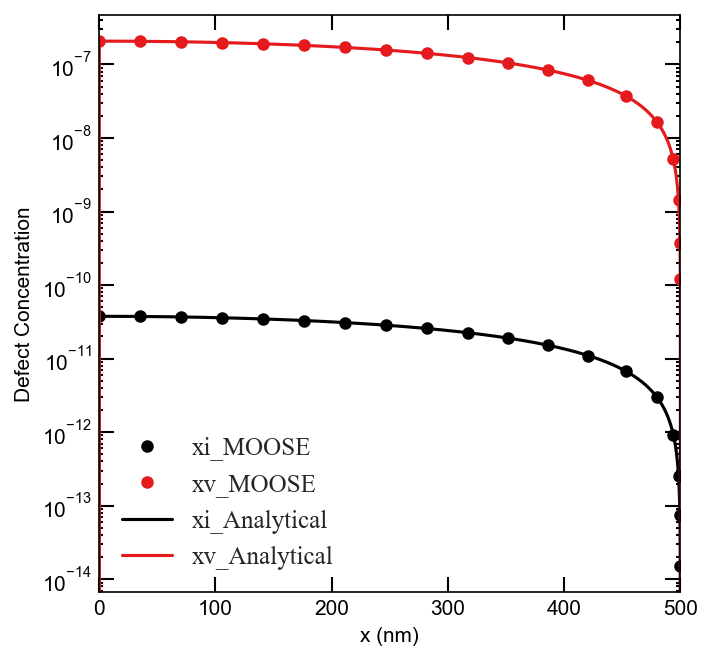
\includegraphics[scale=0.55]{Fig1}
        \caption{A comparison between MOOSE results and the analytical solutions for the fractions of point defects in an irradiated spherical Ni grain with a 500 $nm$ radius. The grain boundary/surface at x = 500 $nm$ is assumed perfect and neutral.}
        \label{figure:concentrations_MOOSE_analytical}
    \end{figure}

 \subsubsection{Concentrations}
 
    The defect concentrations can follow different patterns depending on their properties. Interstitials diffuse to sinks faster than vacancies, and hence their steady-state concentration becomes lower (see Fig. \ref{figure:average_concentrations_neutron_5}a,b).  The evolution of the average fractions of point defects until steady state is captured in Fig. \ref{figure:average_concentrations_neutron_5}.  In these simulations, a production bias of 5\% is assumed and the effects of grain size and dose rate are explored. As expected, longer times are required to reach steady state for larger grains because of the larger diffusion distances. In most cases, also as expected, higher average fractions of defects are associated with larger grains. This is due to the higher surface to volume ratio for smaller grains, which is usually quoted as the origin of radiation tolerance in nanocrystalline materials \citep{was2017,yang2010,demkowicz2011}. However, there are a few exceptions to this latter rule. The transient vacancy concentrations in some of the smaller grains are actually higher than their large counterparts.  For instance, at the low dose rate of 1e-6 $dpa/s$ (Fig. \ref{figure:average_concentrations_neutron_5}a), the transient vacancy concentration at 500 $nm$ is higher than at 5000 $nm$. Moreover, for the high dose rate of 1e-3 $dpa/s$, the transient vacancy concentration at 50 $nm$ is higher than at both 500 $nm$ and 5000 $nm$. This anomaly in the dependence of vacancy accumulation on grain size was observed before in the study by \citep{yang2010}, where lattice kinetic Monte Carlo simulations were employed. This was attributed to the competition between grain boundary absorption of defects and bulk recombination. Both processes have different length and time scales. Nonetheless, the steady state concentrations satisfy the general rule that smaller grains tend to accumulate less defects, which also agrees with \citep{yang2010}.
    
    \begin{figure}[h!]
        \centering
        a)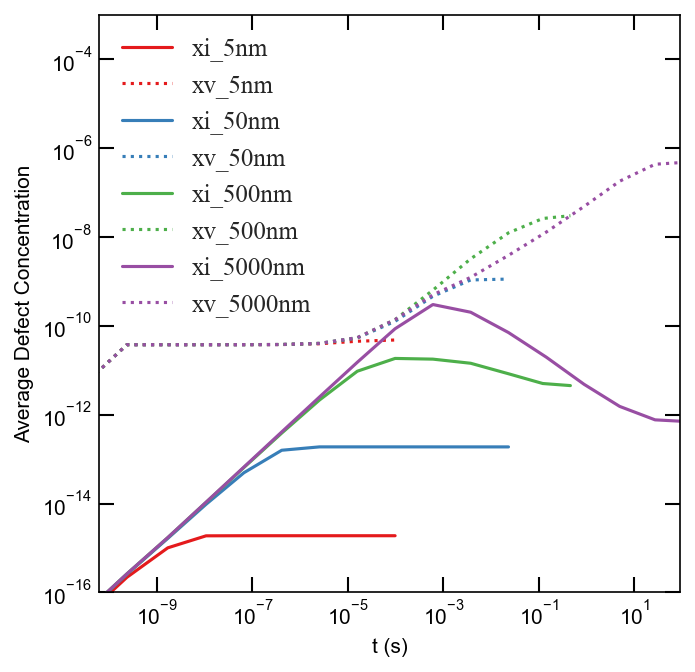
\includegraphics[scale=0.55]{Fig2_a}
        \qquad
        b)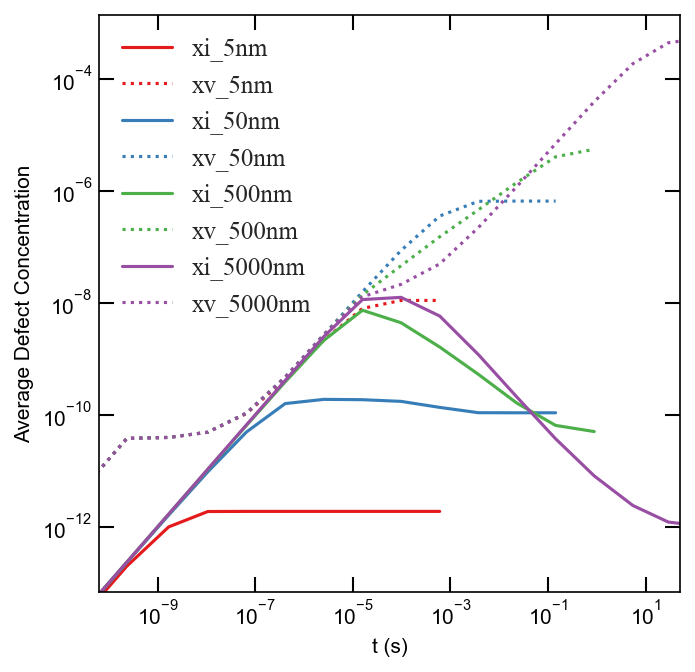
\includegraphics[scale=0.55]{Fig2_b}
        \caption{Time-dependent behavior of average defect concentrations for different grain sizes with a 5\% production bias for a) 1e-6 $dpa/s$ dose rate and b) 1e-3 $dpa/s$ dose rate. Two anomalies for the accumulation of point defects with grain size are observed. First, transient vacancy concentrations are higher in smaller grains during some time intervals, as reported in \citep{yang2010}. Second, transient and steady-state interstitial concentrations decrease with grain size above a critical size (e.g., 1000 $nm$ for the low dose rate and 250 $nm$ for the high dose rate). For the high dose rate, the average steady-state interstitial concentration at 5000 $nm$ is almost equal to its counterpart at 5 $nm$, while its corresponding vacancy concentration is, however, four orders of magnitude higher than its counterpart at 5 $nm$.}
        \label{figure:average_concentrations_neutron_5}
    \end{figure}
    
    The other exception that we report here is a different anomaly related to the accumulation of interstitials. Above a critical grain size, both the transient and steady-state concentrations of interstitials reduce with increasing grain size. For a dose rate of 1e-6 $dpa/s$, the critical size is about 1000 $nm$ (Fig. \ref{figure:average_concentrations_neutron_5}a). The critical size is about 250 $nm$ for a dose rate of 1e-3 $dpa/s$. It is worth noting that for the high dose rate the average interstitial fraction at 5000 $nm$ is almost the same as its counterpart at 5 $nm$, while the corresponding vacancy concentration is about four orders of magnitude higher than its counterpart at 5 $nm$. This anomaly in the interstitial behavior was not detected in \citep{yang2010,demkowicz2011} because of the limitation to small sizes ($<$ 50 $nm$) in those studies.
    
    The effect of grain size on the point defect kinetics resembles to some extent the effect of temperature. If compared to the classical results from homogenized rate-theory \citep{was2017}, which ignores surface, diffusion and size effects, as the grain size changes from small to large, the results show similar trends as if the temperature changes from high to low. This is due to the fact that both factors affect the diffusion kinetics of defects. Nonetheless, the effect of size is even more complicated because of the anomalies discussed above.
    
    The anomaly in the transient behavior of vacancies with grain size is similar to the cases reported in \citep{yang2010}. However, the nature and origin of the anomaly in the behavior of interstitials are different. This is evident from the fact that this new anomaly persists even under steady-state conditions. Hence, a close examination of this anomaly is in order.
    
    The anomaly in the dependence of interstitial accumulation on grain size is associated with an instability that once triggered, different spatial profiles of vacancies and interstitials are established. This is captured in Fig. \ref{figure:time_evolution_5_1e-3_500nm} that depicts the evolution of the interstitial and vacancy profiles with time for a 500 $nm$ planar grain with 1e-3 $dpa/s$ dose rate and 5\% production bias. Initially, the concentrations of both defects increase in the center and reduce at the surfaces, which act as sinks. However, as time progresses, vacancy and interstitial concentrations start to show opposite trends, where vacancies tend to accumulate in the center and interstitials tend to accumulate by the surfaces. This instability appears effectively in relatively large grains ($>$ 100 $nm$) with any nonzero value of production bias (even as low as 0.001\%). The initiation of this instability is attributed to the fact that production bias breaks the symmetry of the balance of point defects leading to non-uniform bulk recombination and non-uniform losses to surfaces (effectively transforming neutral sinks to biased), which eventually results in the development of distinct steady-state profiles for the different point defects.
    
    \begin{figure}[h!]
        \centering
        a)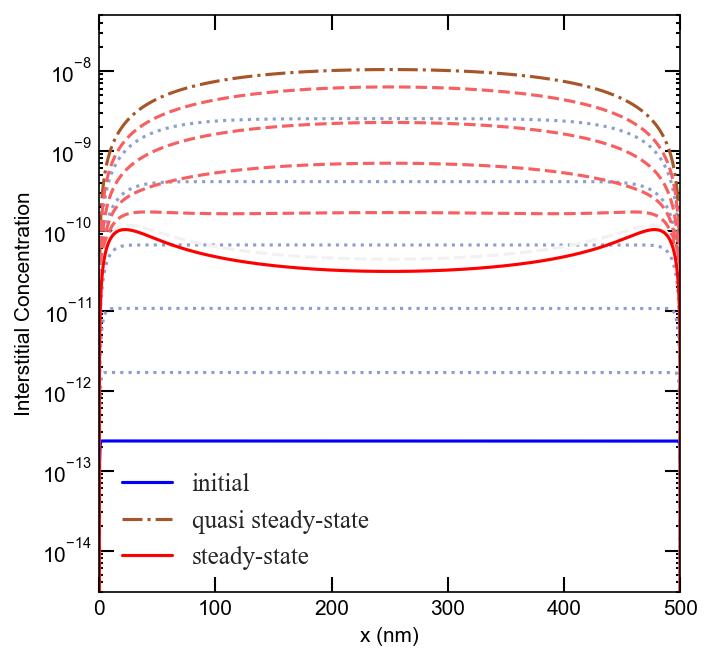
\includegraphics[scale=0.55]{Fig3_a}
        b)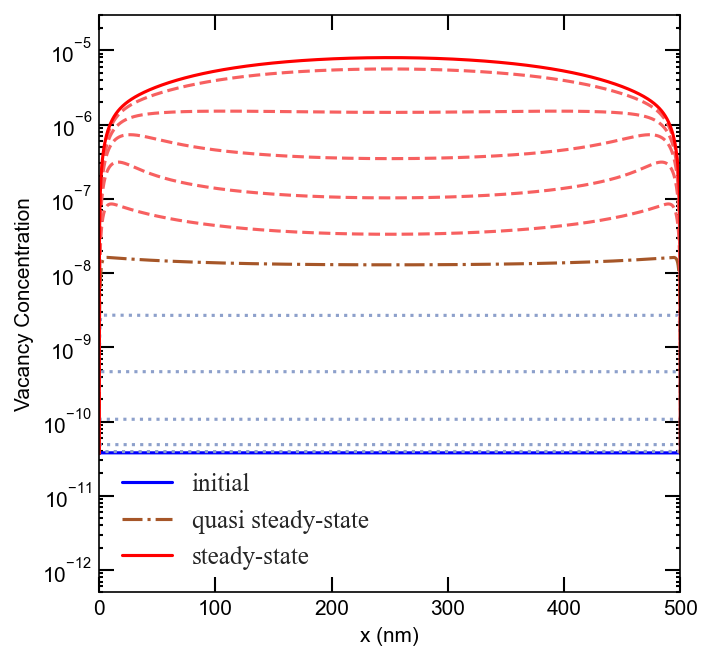
\includegraphics[scale=0.55]{Fig3_b}
        \caption{The evolution of defect concentration profiles at 1e-3 $dpa/s$ and 5\% production bias in a 500 $nm$ slab/equiaxed grain (a planar geometry with two free surfaces/boundaries at both ends), a) for interstitials, b) for vacancies. The calculated times are 1.5764e-3 $sec$ for quasi-steady state condition and 88.8253 $sec$ for steady state condition (see Fig. \ref{figure:average_concentrations_neutron_5}b). }
        \label{figure:time_evolution_5_1e-3_500nm}
    \end{figure}
    
    The opposite trends of vacancies and interstitials arise because of their distinct dynamics. Interstitials are produced at a lower rate than vacancies. Also, interstitials are faster than vacancies. If one runs a hypothetical simulation with those conditions reversed, the steady-state spatial profiles of vacancies and interstitials will also be reversed.
    
    Since the diffusion coefficients are temperature dependent, the Di/Dv ratio changes with temperature. To investigate the effect of diffusivity ratio/temperature, several simulations were conducted for different temperatures with a production bias of 5\% and a production rate of 1e-3 $dpa/s$ in a 1000 $nm$ grain. The results are presented in Fig. \ref{figure:concentrations_high_neutron_5_temperature}. As evident from the figure, there is a critical ratio ($\approx$33 for Ni) below which the instability is suppressed. In other words, there is a critical temperature only below which the instability develops.
    
    \begin{figure}[h!]
        \centering
        a)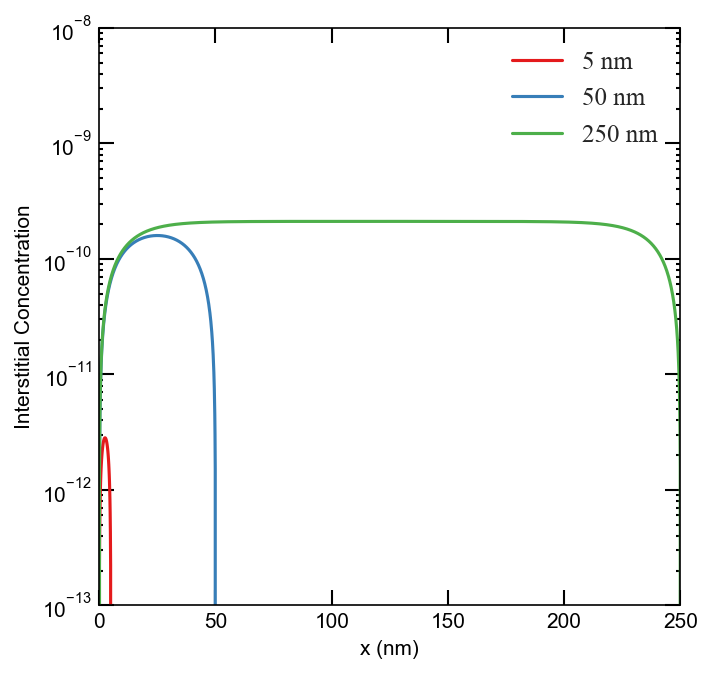
\includegraphics[scale=0.55]{Fig4_a}\\
        b)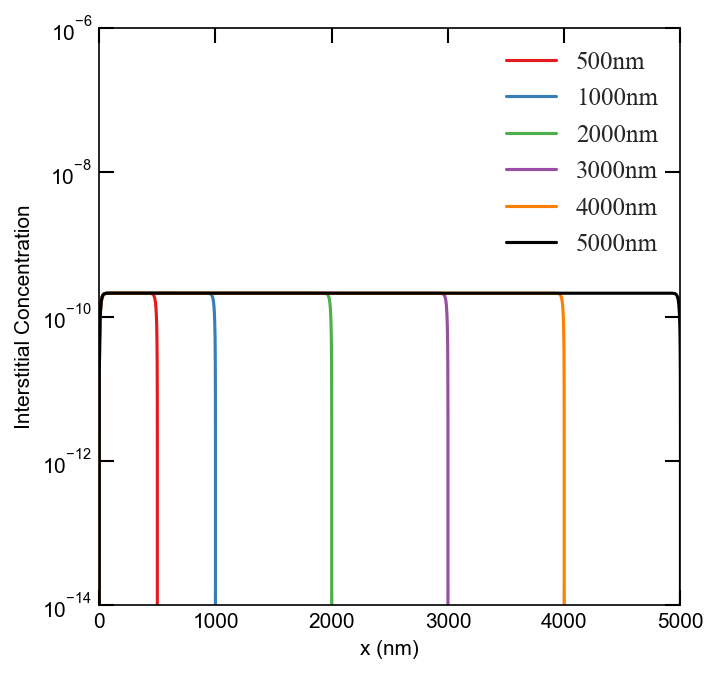
\includegraphics[scale=0.35]{Fig4_b}
        c)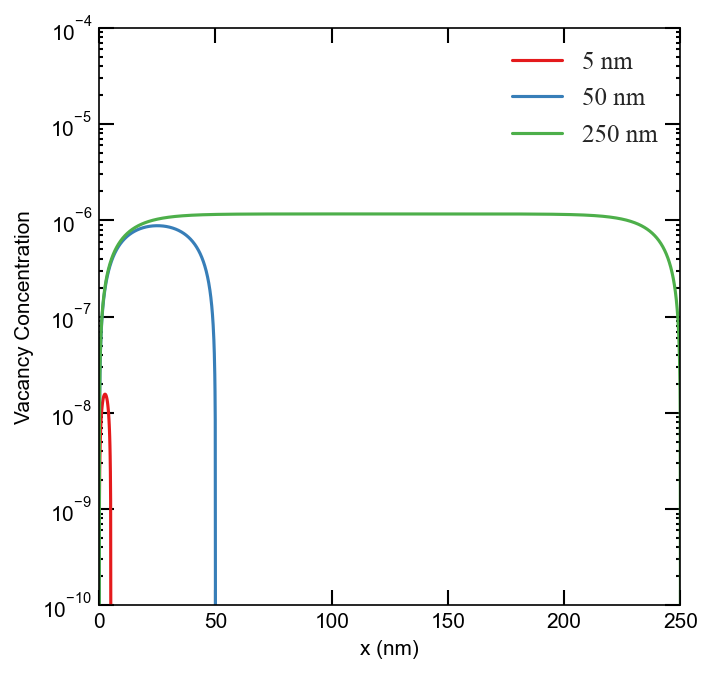
\includegraphics[scale=0.35]{Fig4_c}
        
\includegraphics[scale=0.35]{Fig4_legend}
        \caption{a) The change of diffusivity ratio, $D_i/D_v$, with temperature. Effect of temperature/diffusivity ratio on the development of the instability at 1e-3 $dpa/s$ and 5\% production bias in a 1000 $nm$ slab/equiaxed grain, b) for interstitials, c) for vacancies.}
        % \caption{Effect of grain size on the steady-state concentration profiles of point defects at 1e-3 $dpa/s$ in the absence of production bias. Upper row: interstitials in a) fine grains, b) coarse grains. Lower row: vacancies in c) fine grains, d) coarse grains. The steady-state concentrations of point defects increase with grain size, but this increase saturates above a size of 250 $nm$. }
        \label{figure:concentrations_high_neutron_5_temperature}
    \end{figure}
    
    This instability is also sensitive to grain size, dose rate, and production bias. This is demonstrated in Figs. \ref{figure:concentrations_neutron_5} and \ref{figure:3D_concentrations_neutron_1e-6}. In Fig. \ref{figure:concentrations_neutron_5}, the effect of grain size is shown for two different dose rates with a production bias of 5\%. In all cases, the steady-state vacancy concentration increases with grain size and is highest in the center. The vacancy concentration gradients in the vicinity of surfaces increases with dose rate. On the other hand, the steady-state interstitial concentration initially follows the same trend as the vacancy concentration up to a critical size, above which the trend is reversed, i.e., interstitial concentration decreases with grain size. This critical size is 250 $nm$ for a dose rate of 1e-3 $dpa/s$ and 1000 $nm$ for a dose rate of 1e-6 $dpa/s$. This is consistent with Fig. \ref{figure:average_concentrations_neutron_5} and hence this instability is indeed the origin of the size anomaly discussed above. The production bias also plays an important rule. Using 3D plots, Fig. \ref{figure:3D_concentrations_neutron_1e-6} demonstrates the combined effects of size, dose rate, and production bias. Generally speaking, the critical size reduces with dose rate and production bias.
    
    It is worth mentioning that such instability will render irradiation damage more pronounced. This due to the fact that the pattern that develops based on this instability favors the separation of vacancies and interstitials. Therefore, it will enhance the possibility of clustering of different point defects into distinct extended defects. Namely, vacancies at the center of the domain will cluster into voids or vacancy loops, while interstitials close to the boundaries will form dislocation loops. It is also interesting to note that this instability is suppressed in nano-grains (with sizes less than 100 $nm$). This provides a new insight into the stability of nano-materials, i.e., such materials support the development of point defect patterns that limit the formation of extended defects.

    It is unfeasible to measure experimentally the densities of single point defects in a direct way. However, our results here can be indirectly validated by the well-known existence of void denuded zones close to grain boundaries. Since the instability in our results show accumulation of interstitials and depletion of vacancies adjacent to GBs, it is expected that void formation will be suppressed under such conditions.
    
    Additionally, the dependence of the severity of radiation damage on grain size predicted here agrees with the recent experimental study by \citep{mao2019}. In that study, the sink strength of nano-GB is quantitatively investigated in the nano-grained Cu and dilute Cu-W alloys with the average grain size ranging from ~20 to ~500 $nm$ by ~300 $keV$ He ions irradiation at room temperature and 673 $K$. The irradiation induced void volume ratio, size and distribution are confirmed to strongly depend on the grain size and irradiation temperature. It was found that there is a critical size below which the samples are completely radiation resistant and almost no voids form. Moreover, such full radiation tolerance was only achieved at the high temperature but not the low temperature. Those findings are clearly in agreement with our prediction here.
    
    Lastly, it is noteworthy that this instability is different from the Turing instability usually invoked to explain void/bubble superlattices formation in irradiated solids \citep{noble2020,ghoniem2001,krishnanOct1980,gao2018}. Turing instability can be inferred from linear stability analysis and depends on the ratio and/or anisotropy of diffusion coefficients. The current instability, however, is nonlinear, surface induced, and size regulated.

    \begin{figure}[h!]
        \centering
        a)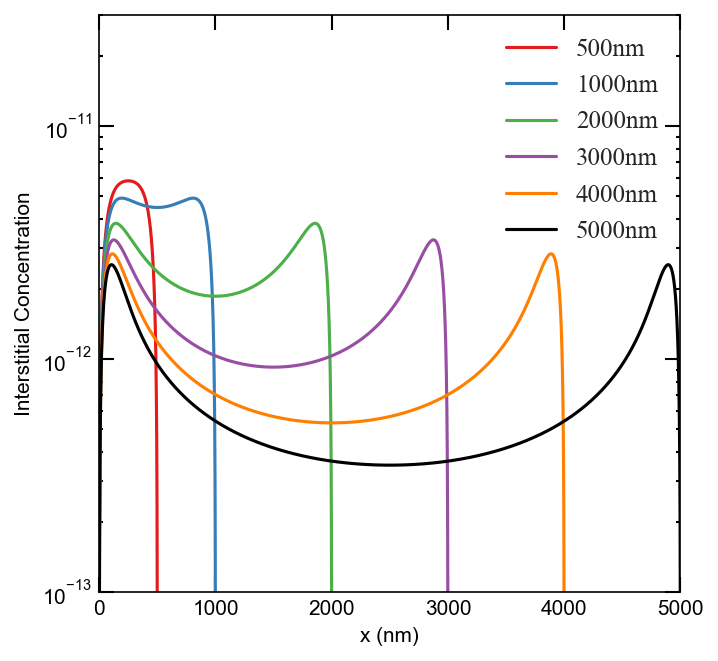
\includegraphics[scale=0.55]{Fig5_a}
        b)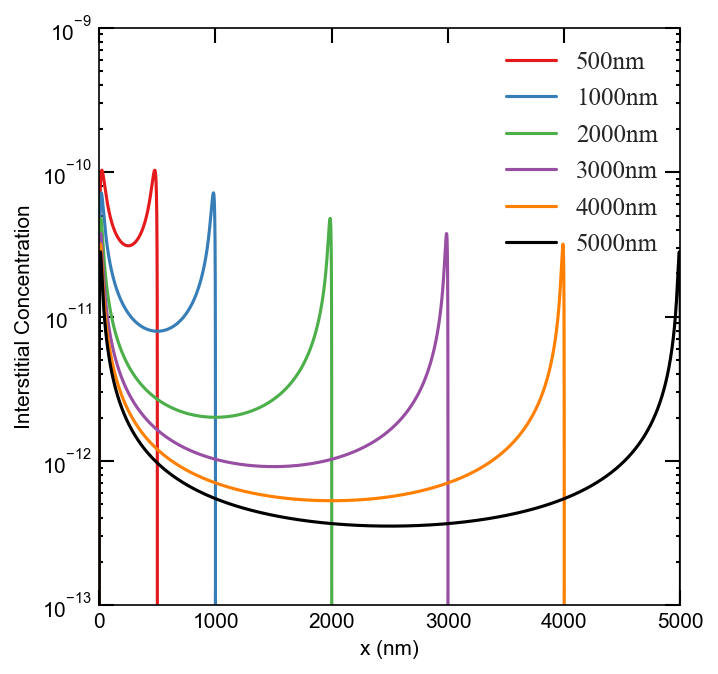
\includegraphics[scale=0.55]{Fig5_b}
        c)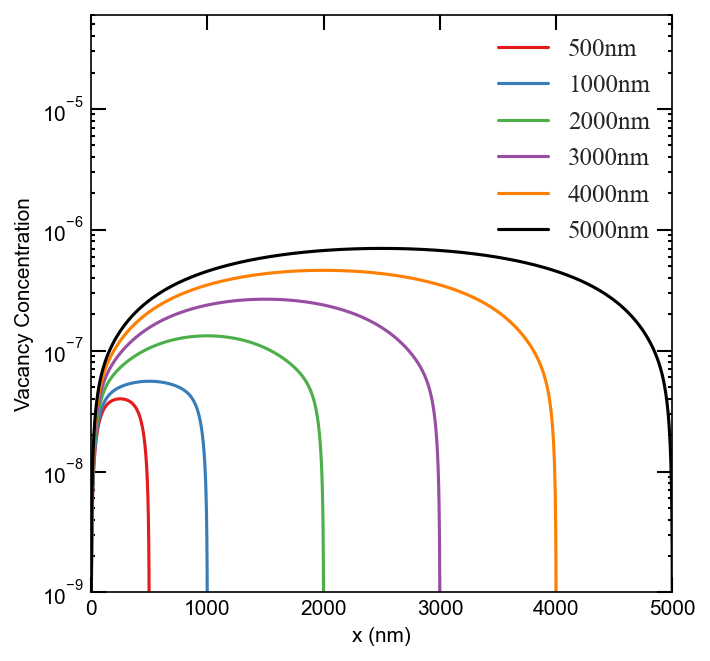
\includegraphics[scale=0.55]{Fig5_c}
        d)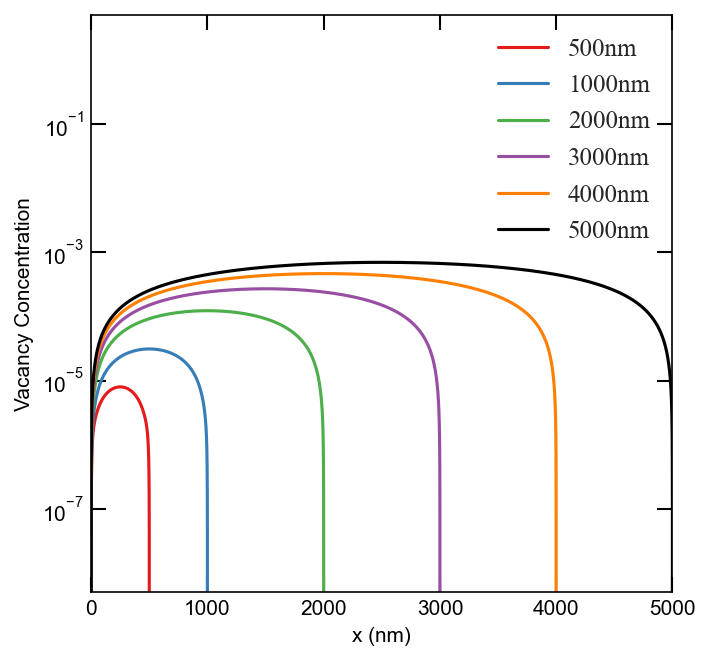
\includegraphics[scale=0.55]{Fig5_d}
        \caption{Effect of grain size on the steady-state concentration profiles of point defects at 5\% production bias. Upper row: interstitials a) low dose rate (1e-6 $dpa/s$), b) high dose rate (1e-3 $dpa/s$). Lower row: vacancies c) low dose rate (1e-6 $dpa/s$), d) high dose rate (1e-3 $dpa/s$).} %Note the drastic contrast with the results presented in Fig. \ref{figure:concentrations_micro_nano_neutron_5_1e-3} in the absence of production bias.}
        \label{figure:concentrations_neutron_5}
    \end{figure}
   \begin{figure}[htb!]
        \centering
        a)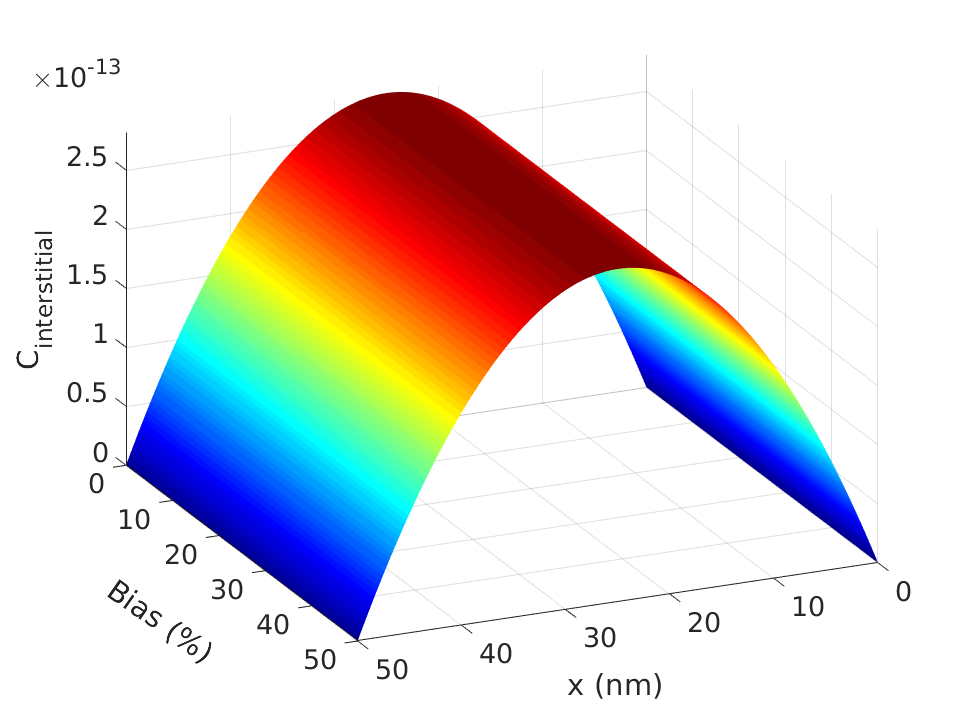
\includegraphics[scale=0.3]{Fig6_a}
        b)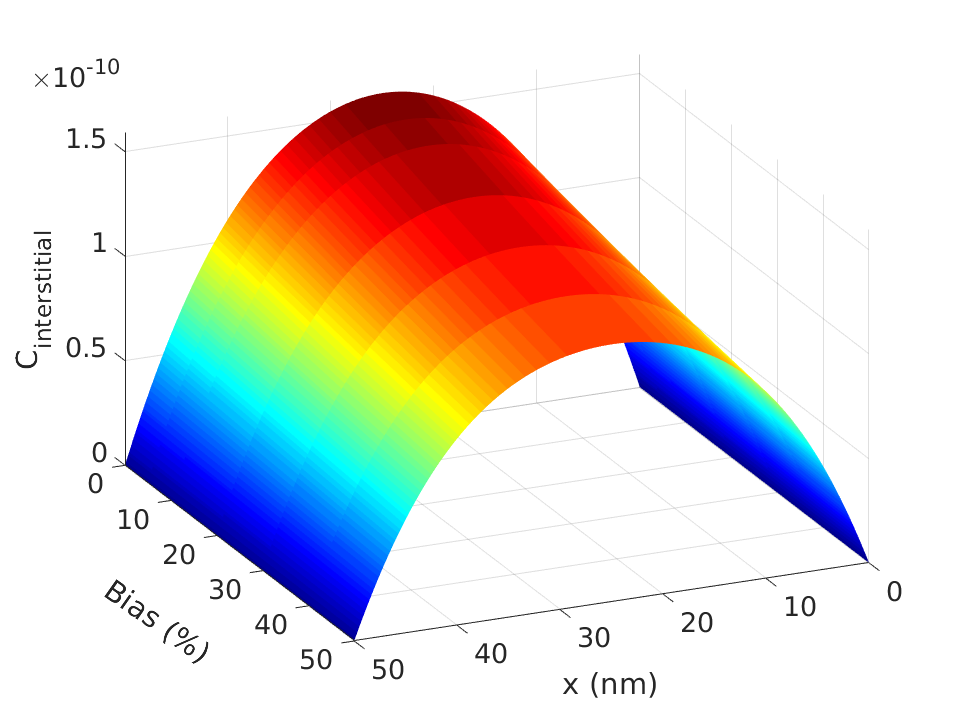
\includegraphics[scale=0.3]{Fig6_b}
        c)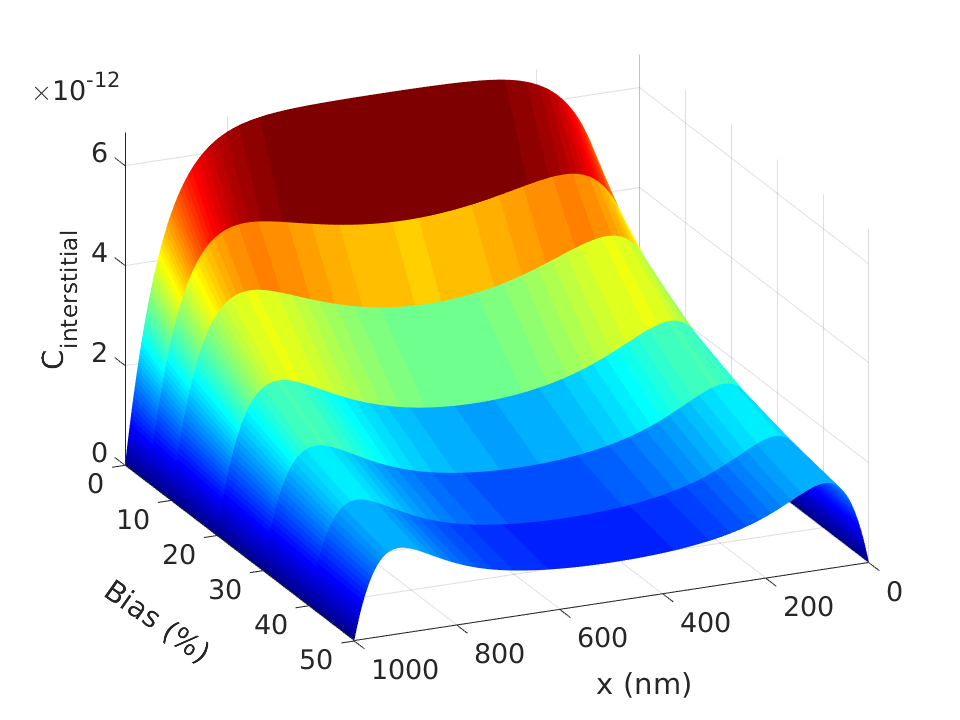
\includegraphics[scale=0.3]{Fig6_c}
        \qquad
        d)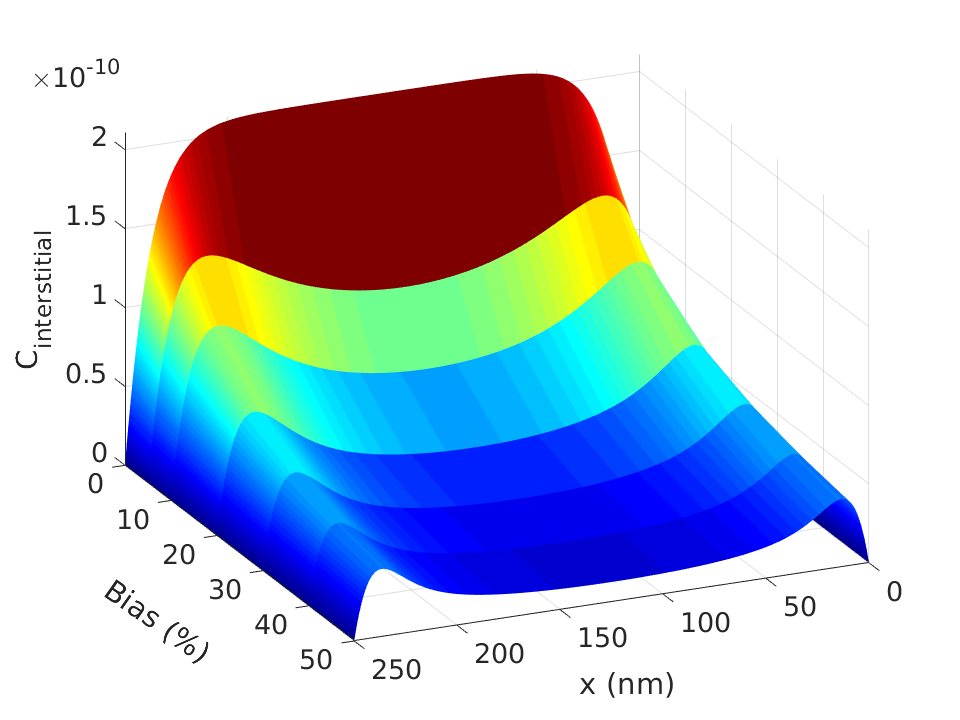
\includegraphics[scale=0.3]{Fig6_d}
        \caption{An illustration of the combined effects of size, dose rate, and production bias on the steady-state profiles of interstitials. Change of interstitial concentration profiles with production bias for a) low dose rate (1e-6 $dpa/s$) and 50 $nm$ grain, b) high dose rate (1e-3 $dpa/s$) and 50 $nm$ grain, c) low dose rate (1e-6 $dpa/s$) at the critical grain size ($\approx$1000 $nm$), d) high dose rate (1e-3 $dpa/s$) at the critical grain size ($\approx$250 $nm$).}
        \label{figure:3D_concentrations_neutron_1e-6}
    \end{figure}

\subsubsection{Vacancy Supersaturation}

    Void formation is one of the most studied processes in irradiated solids \cite{was2017,noble2020,ghoniem2001,krishnanOct1980,gao2018}. This process often takes place whenever a vacancy supersaturation develops in irradiated solids, i.e., when the vacancy concentration is much higher than the equilibrium concentration. Vacancies tend to cluster together into voids to lower the overall free energy of the system. Void formation usually leads to void swelling. The presence of voids and the dimensional change associated with void swelling drastically alter the thermo-mechanical properties of materials.  
    
    In this section, we investigate the effects of surface, size, dose rate, and production bias on the development of vacancy supersaturation in irradiated solids. An effective vacancy supersaturation, $S_v$, can be estimated from the following equation \citep{was2017},

    \begin{equation}
        \begin{aligned}
        &S_v=\frac{D_vC_v-D_iC_i}{D_vC_v^e}\\
        \end{aligned}
    \end{equation}
    The effective vacancy concentration increases with vacancy concentration and reduces with interstitial concentration. 
    
    Fig. \ref{figure:vacancy_supersaturation_neutron} presents the effects of dose rate, production bias, and size on vacancy supersaturation. First, the spatial dependence of vacancy supersaturation as function of size for two different dose rates is captured in the 2D plots. Following the vacancy concentration (recall Fig. \ref{figure:time_evolution_5_1e-3_500nm}), the maximum vacancy supersaturation is largest in the center. In general, vacancy concentration increases with dose rate, production bias, and size. For the same size, temperature, and production bias, the dependence on dose rate is almost linear. However, the dependence on size or production bias is non-linear. This is clear from the 3D plots that shown the combined effects of size and bias. The effect of size is detailed in Fig. \ref{figure:center_vacancy_supersaturation_neutron} that depicts the change of the maximum vacancy supersaturation with size at a dose rate of 1e-6 $dpa/s$ and 5\% bias. As obvious from the figure, the development of vacancy supersaturation is suppressed in submicron grains, while facilitated in large grains. Not only vacancy concentration increases with grain size, but its rate of increase also climbs with size. It is noteworthy that the increase of vacancy concentration becomes more apparent above the critical size. For instance, the ratio between the maximum vacancy concentration at 500 $nm$ compared to 50 $nm$ is 67.6, while the corresponding ratio at 5000 $nm$ compared to 500 $nm$ is 89.97. This supports our earlier prediction that the bias-enabled, surface-induced, and size regulated instability and developed pattern exaggerate irradiation damage.

    \begin{figure}[h!]
        \centering
        a)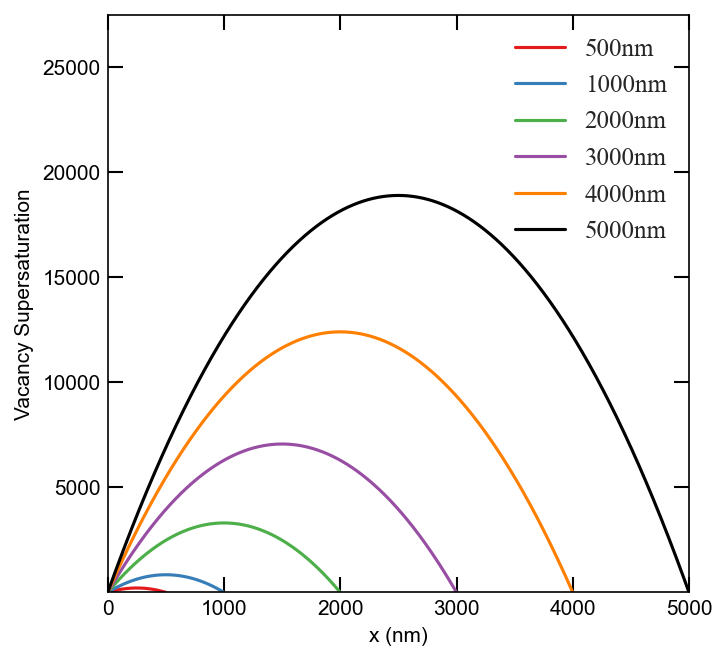
\includegraphics[scale=0.55]{Fig7_a}
        b)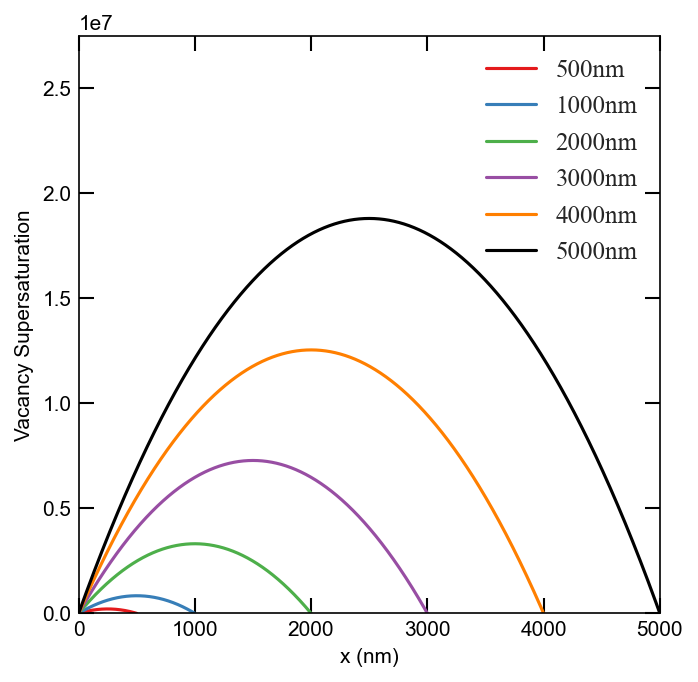
\includegraphics[scale=0.55]{Fig7_b}
        \qquad
        c)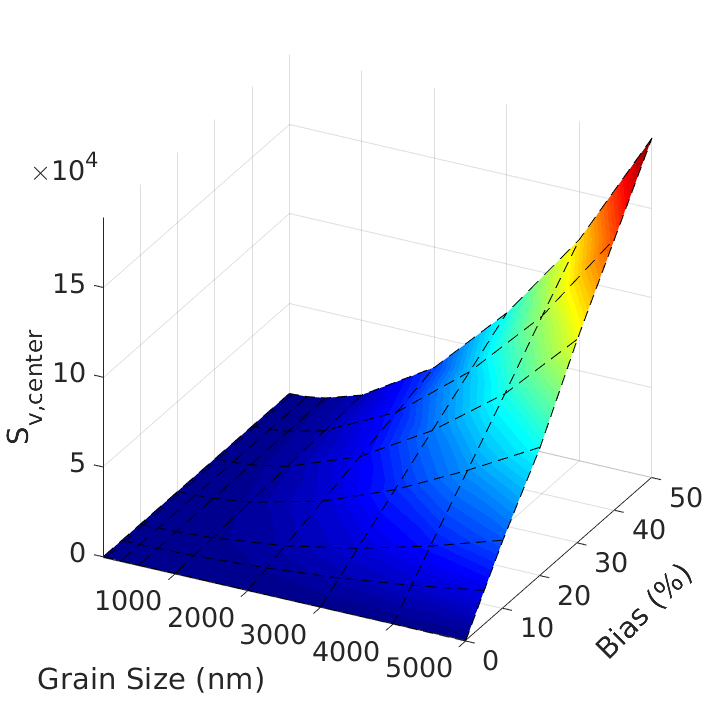
\includegraphics[scale=0.35]{Fig7_c}
        d)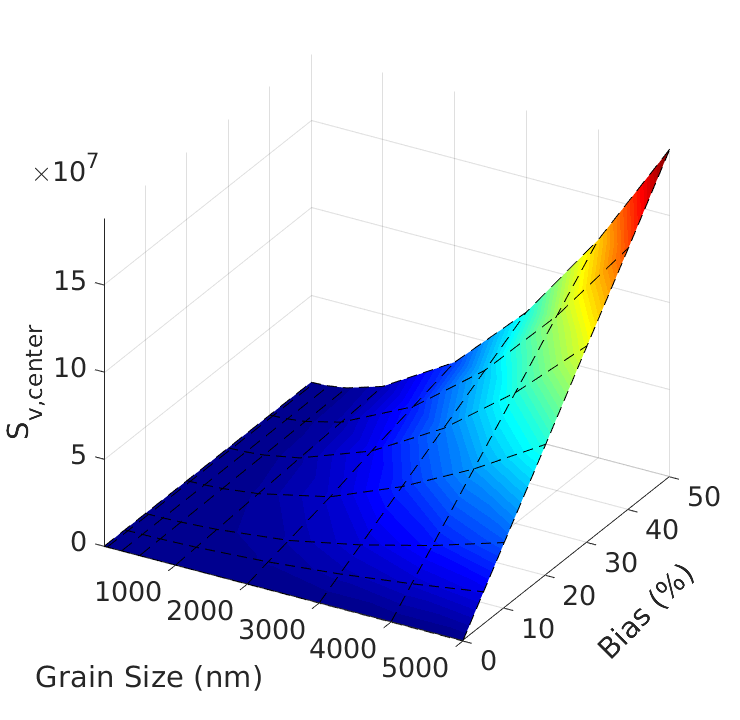
\includegraphics[scale=0.35]{Fig7_d}
        \caption{The effects of dose rate, production bias, and size on vacancy supersaturation. Upper row: Vacancy supersaturation profiles for 5\% production bias for a) low dose rate (1e-6 $dpa/s$), and b) high dose rate (1e-3 $dpa/s$). Lower row: Maximum vacancy supersaturation for different values of production bias and grain size for c) low dose rate (1e-6 $dpa/s$), and d) high dose rate (1e-3 $dpa/s$).}
        \label{figure:vacancy_supersaturation_neutron}
    \end{figure}
    
    \begin{figure}[h!]
        \centering
        a)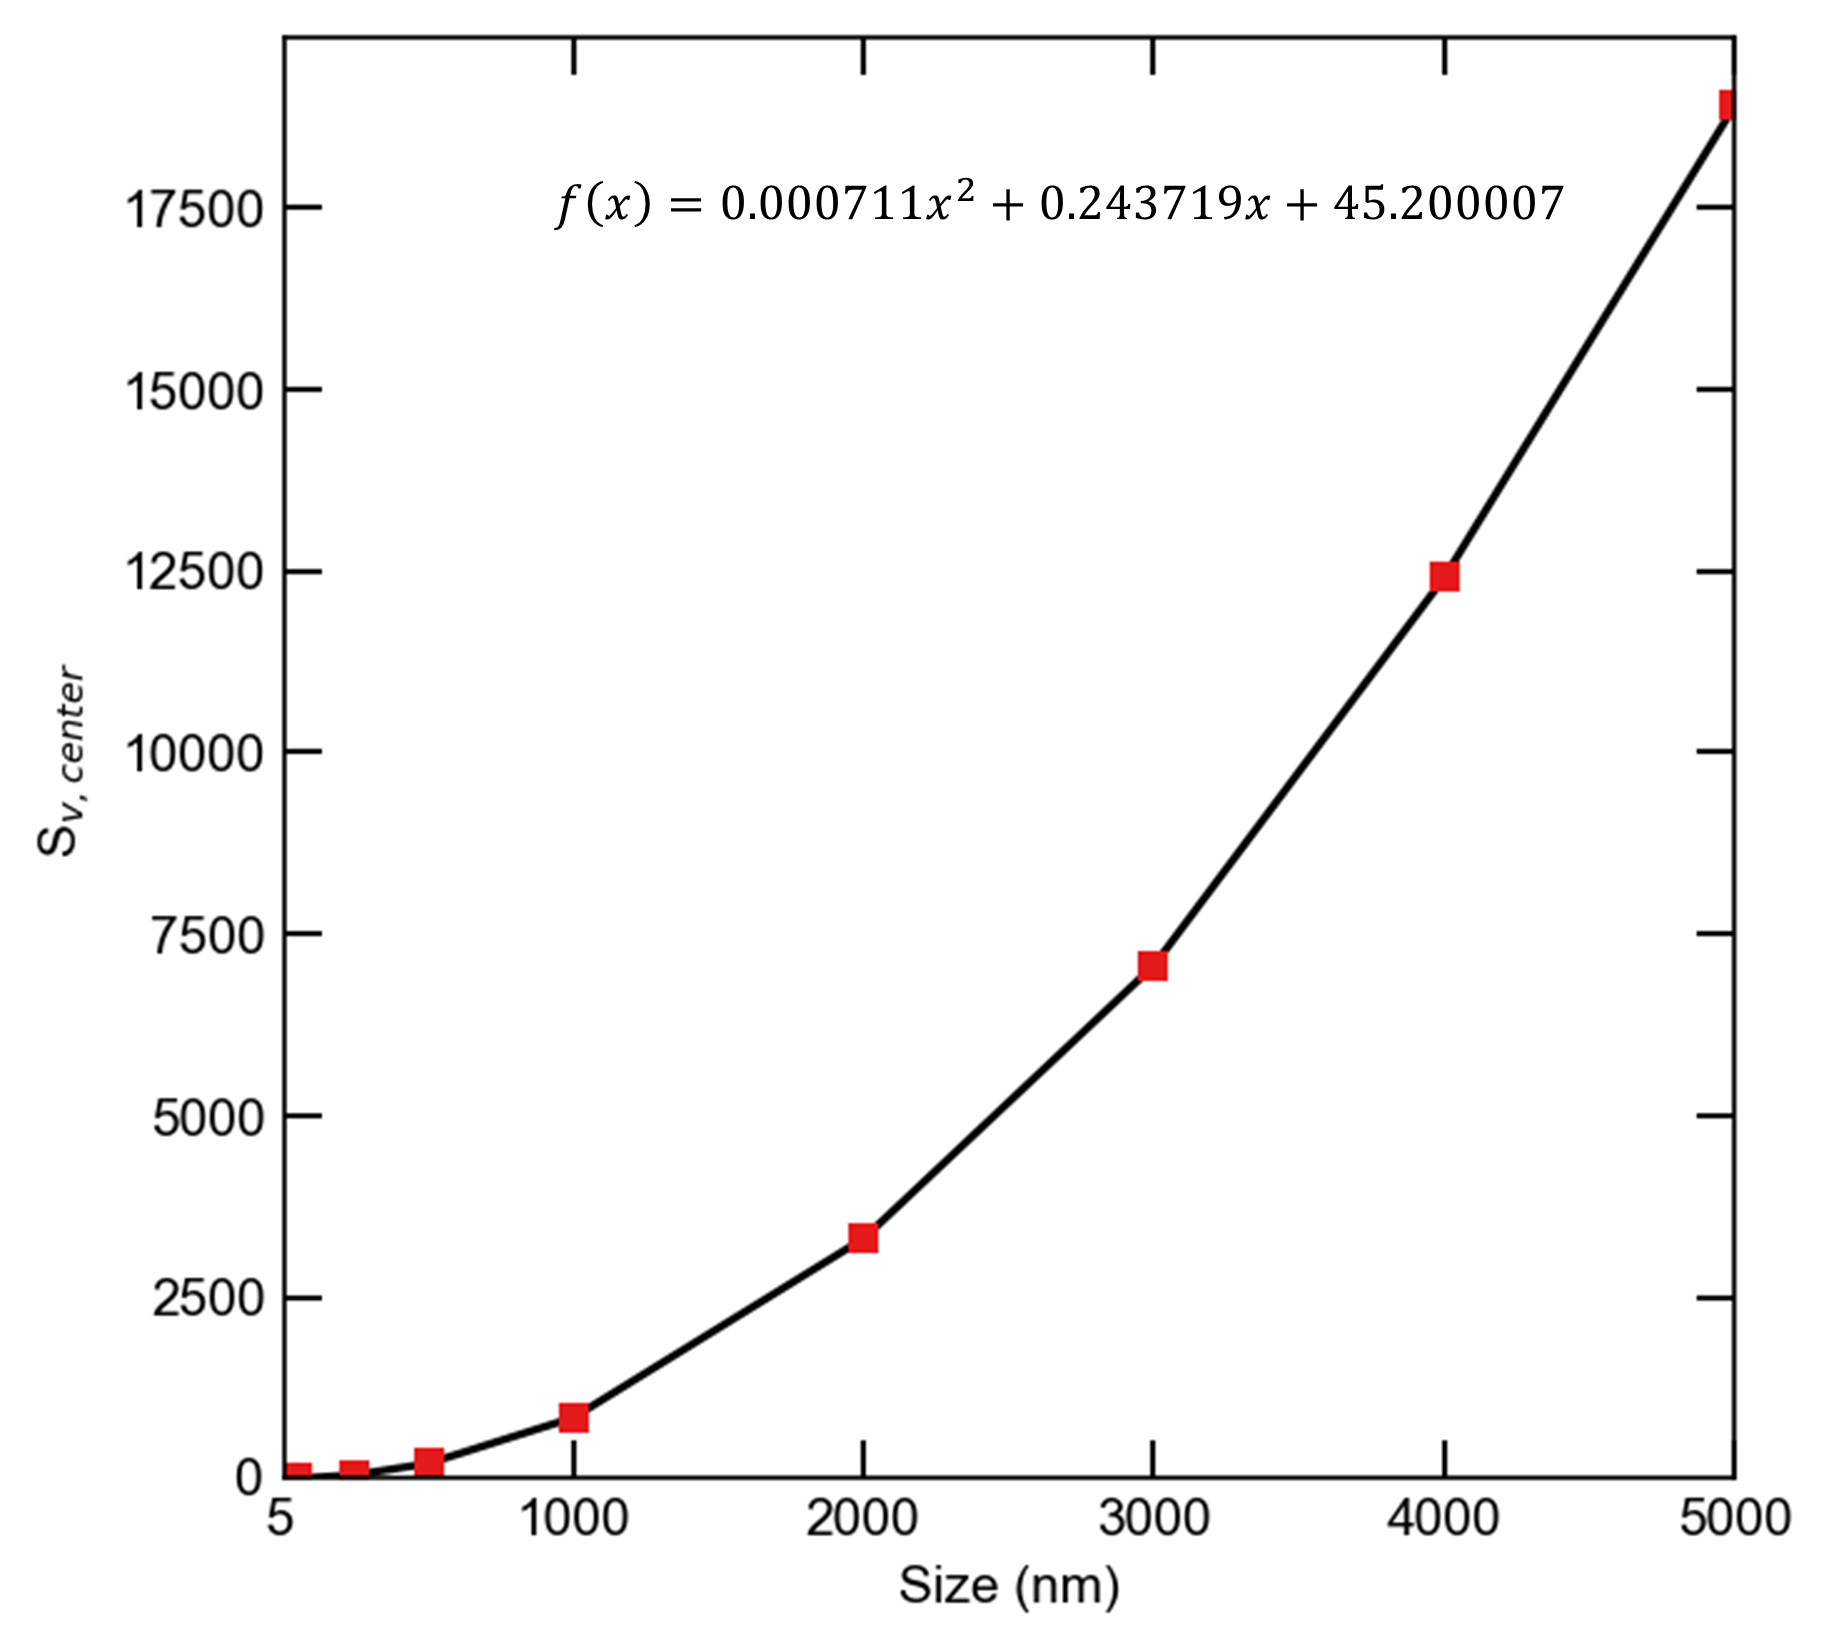
\includegraphics[scale=0.55]{Fig8_a}
        \\
        \qquad
        b)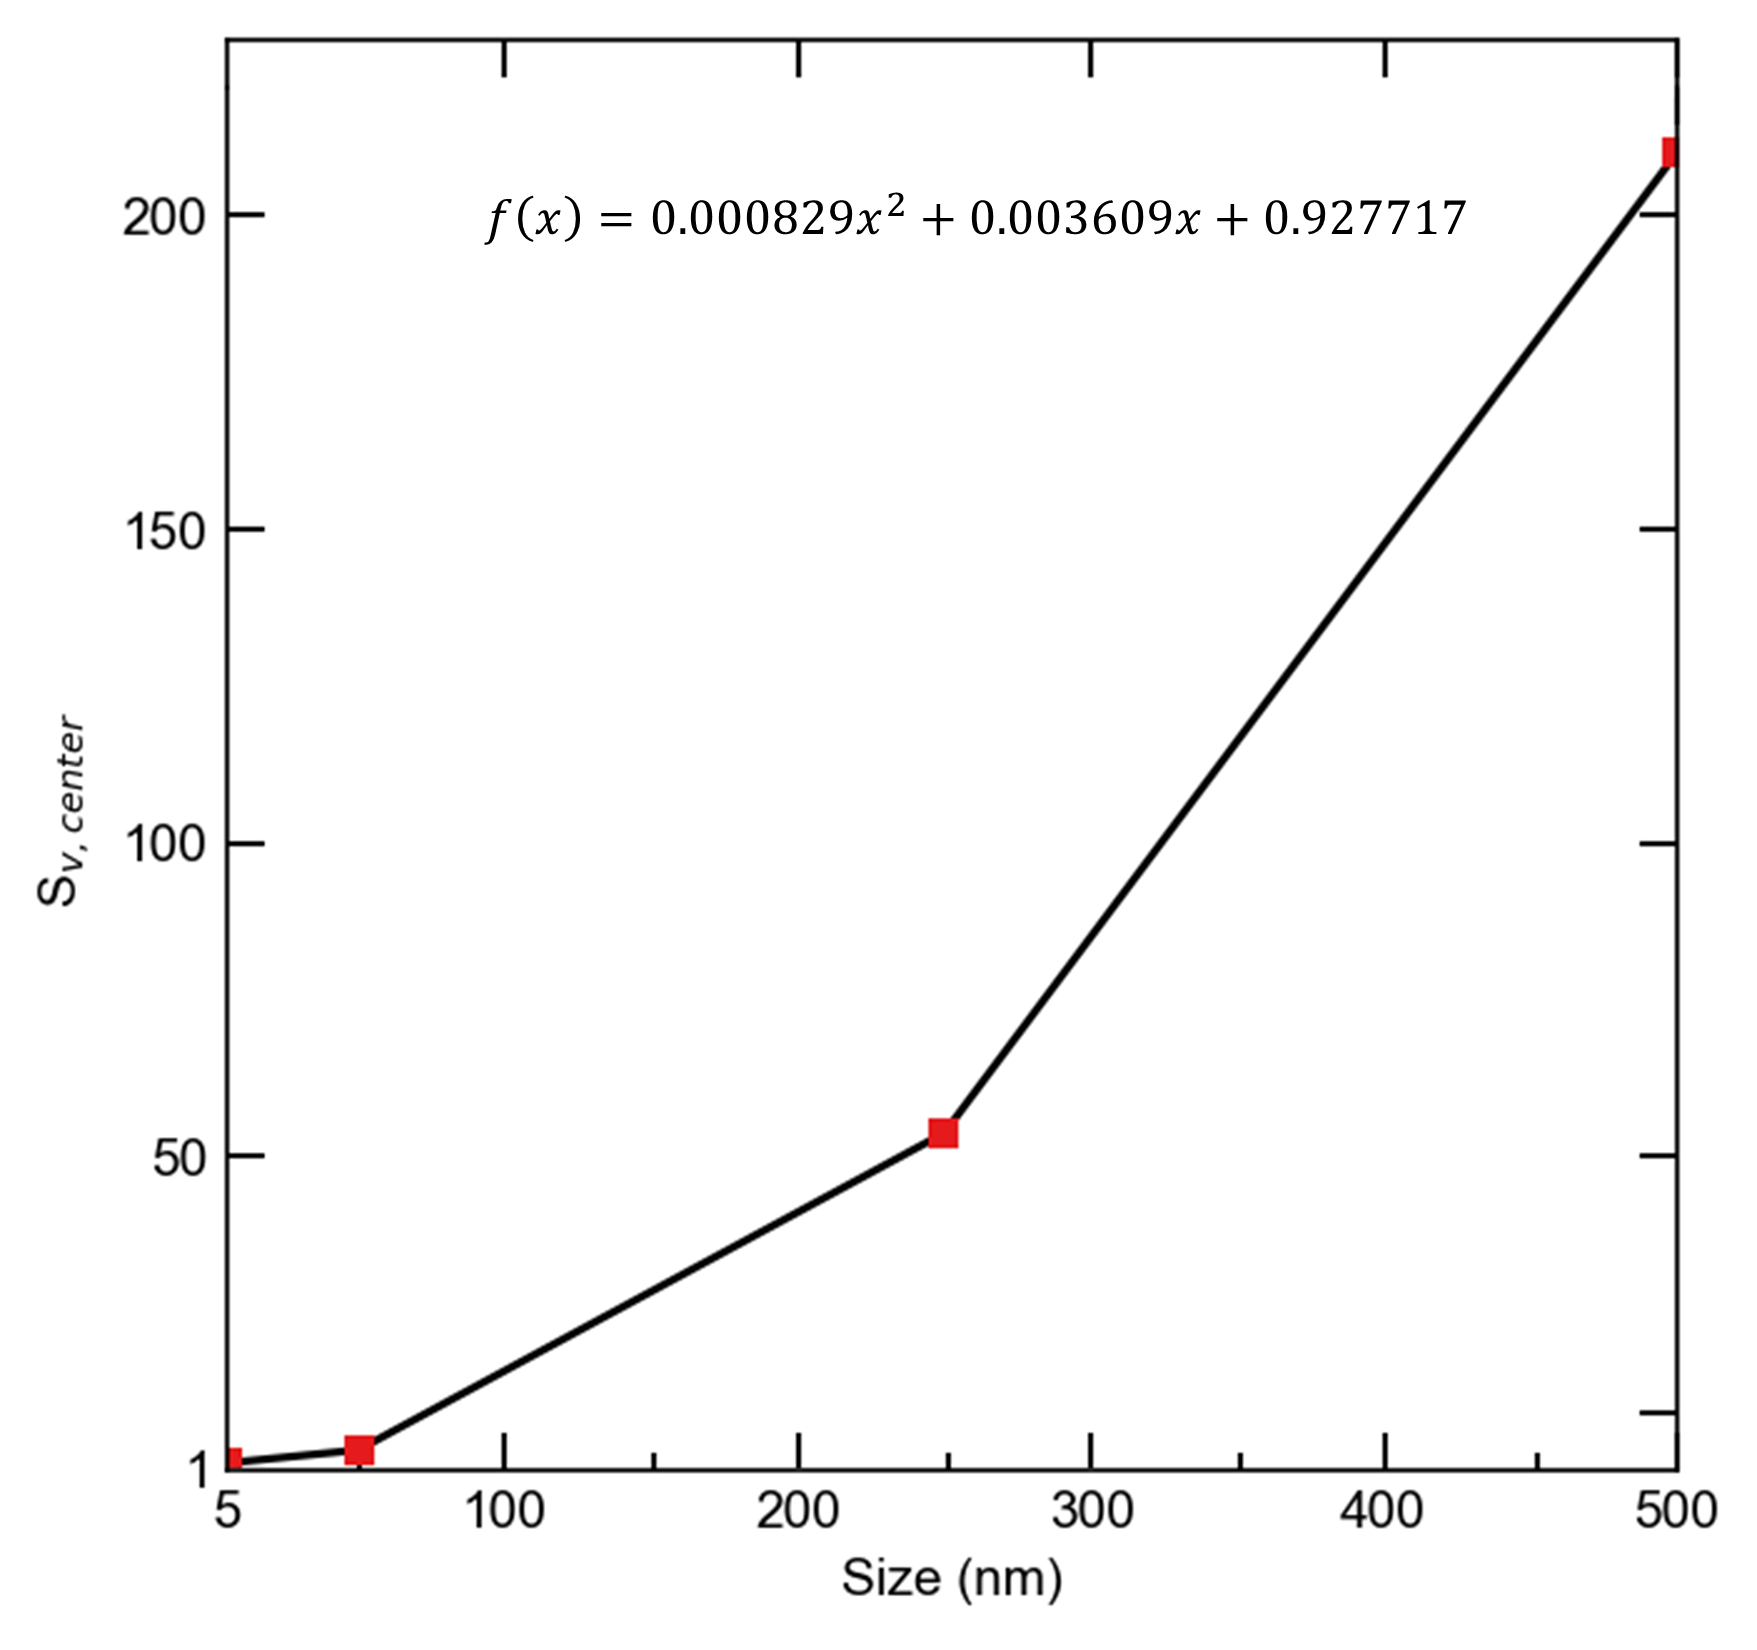
\includegraphics[scale=0.55]{Fig8_b}
        c)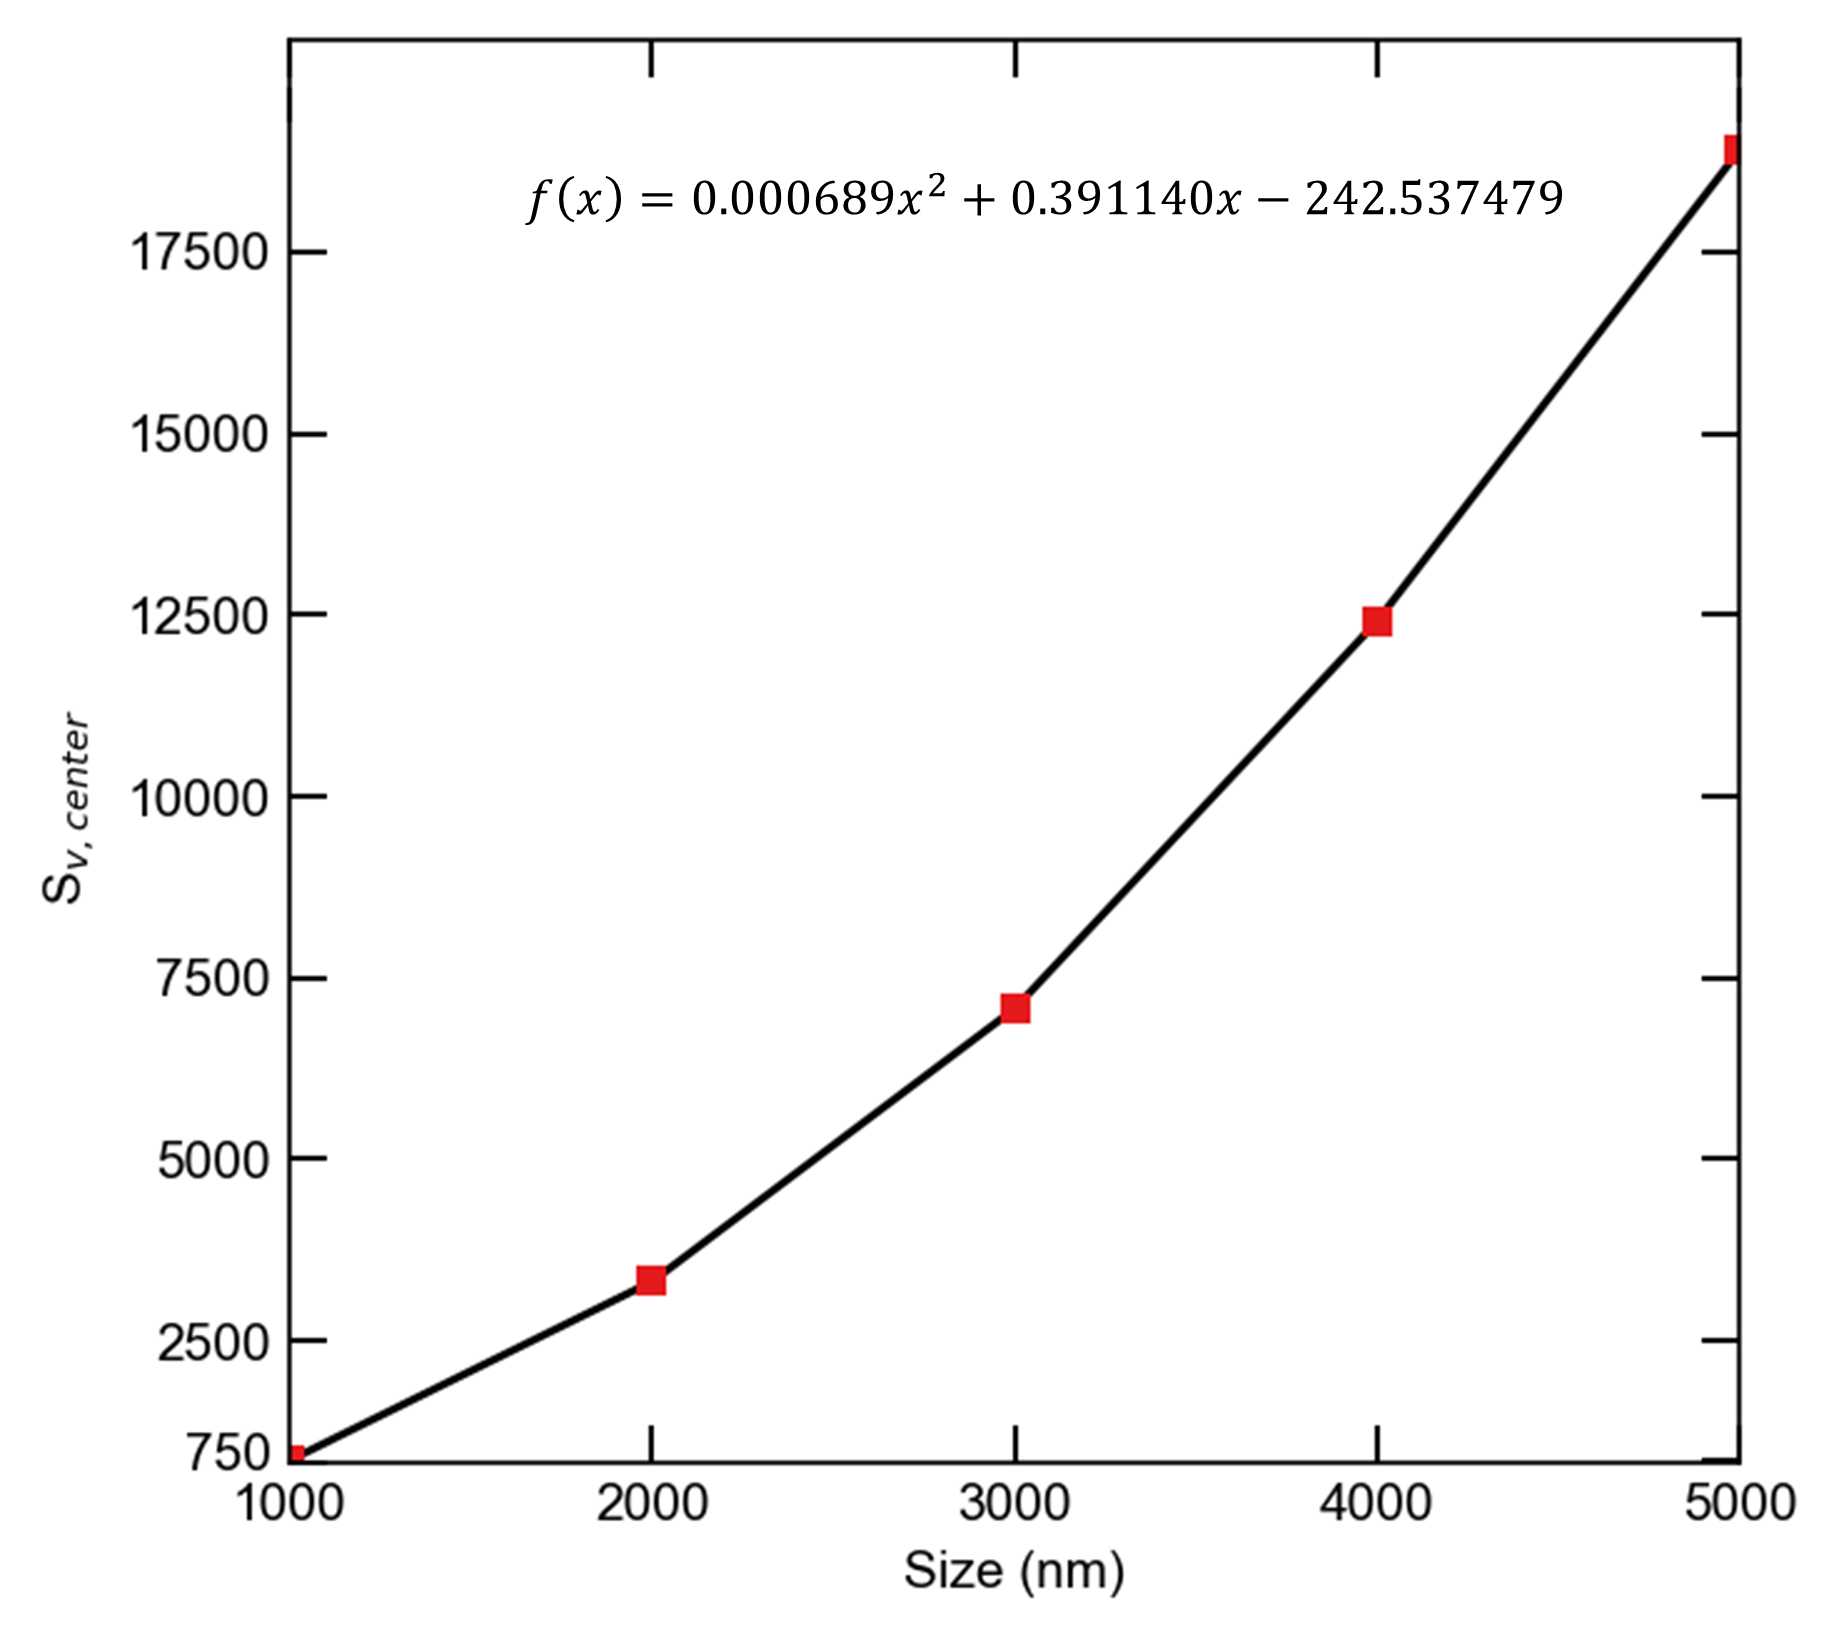
\includegraphics[scale=0.55]{Fig8_c}
        \caption{The effect of size on maximum vacancy supersaturation at a dose rate of 1e-6 $dpa/s$ and 5\% production bias. (a) whole size range, (b) submicron sizes (c) micro sizes. The maximum vacancy supersaturation increases with grain size and the rate of increase also rises with grain size. The effect of grain size is more pronounced above the critical size (1000 $nm$). The fitting equations are valid for sizes between 5 and 5000 $nm$.\\}
        \label{figure:center_vacancy_supersaturation_neutron}
    \end{figure}

\subsubsection{Grain Boundary Sink Strength}
    The sink reaction term in Eq. \ref{equation:point_defect_equations_sink_strength} represents the total loss of point defects to sinks in the bulk such as voids and dislocations. It can be written in expanded form as below,

    \begin{equation}
      \begin{aligned}
        &k^2DC=(k_d^2 + k_v^2)DC
      \end{aligned}
    \end{equation}\\
    where ${k_d^2}$ is sink strength for dislocations in $m^{-2}$, $ {k_v^2}$ is sink strength for voids in ${m^{-2}}$,
    
    Similarly, grain boundary sink strength can be calculated by considering total flow of point defect to grain boundary.

    \begin{equation}
      \begin{aligned}
        &F=Z_{gb}DC_0\\
        &Z_{gb}=\frac{F}{DC_0}
      \end{aligned}
      \end{equation}\\
    where ${F}$ is total flow at grain boundary, ${Z_{gb}}$ is grain boundary sink strength, ${D}$ is diffusion coefficient and ${C_0}$ is defect concentration at the domain center.
    
    The total flow at boundary is equal to multiplication of surface area and current as below,

    \begin{equation}
      \begin{aligned}
        &F=-\bigg(4\pi r^2D\frac{\partial C(r)}{\partial r}\bigg)_{r=a}
      \end{aligned}
    \end{equation}
    
    The total grain boundary sink strength, ${k^2_{gb}}$ is calculated by multiplying ${Z_{gb}}$ by the grain density, ${\rho_{gb}}$. \citep{heald1977}\\
    \begin{equation}
      \begin{aligned}
        &\rho_{gb}=\frac{6}{\pi d^3}\\
        &k^2_{gb}=\rho_{gb}Z_{gb}
      \end{aligned}
    \end{equation}\\
    where ${d}$ is diameter of the grain, ${d=2a}$.
  
    For the benchmark problem of a spherical grain described earlier, grain boundary sink strengths, $Z_{gb}$ and $k^2_{gb}$, are calculated analytically by substituting Eq. \ref{equation:spherical_grain_analytical_solution} into the expressions above. First, the concentration at the grain center and total flow at the grain boundary are expressed in terms of the production rate and the bulk sink strength, $k^2$ as follows \cite{heald1977}.\\

    \begin{equation}
      \begin{aligned}
        &C_0=C(r=0)=\frac{K_0}{Dk^2}\bigg(1-\frac{ka}{\sinh{ka}}\bigg)\\\\
        &F=-\bigg(4\pi r^2D\frac{\partial C(r)}{\partial r}\bigg)_{r=a}=\frac{4\pi aK_0}{k^2}\bigg(ka\coth{ka}-1\bigg)
      \end{aligned}
    \end{equation}\\
    
    Then, grain boundary sink strengths are given by
    
    \begin{equation}
      \begin{aligned}
        &Z_{gb}=4\pi a\bigg(\frac{ka\cosh ka-\sinh ka}{\sinh ka-ka}\bigg)\\
        &k^2_{gb}=\frac{12}{d^2}\bigg(\frac{ka\cosh ka-\sinh ka}{\sinh ka-ka}\bigg)
      \end{aligned}
      \label{equation:grain boundary sink strengths}
    \end{equation}

    Eq. (\ref{equation:grain boundary sink strengths}) predicts the same individual (for a grain boundary) and total sink strengths for both point defects in the presence of neutral bulk sinks. However, dislocations are known to be biased towards the absorption of more interstitials than vacancy because of their stress field.  In that case, grain boundary sink strengths for different defect types can be calculated by using appropriate diffusion coefficient ($D$), bulk sink strength ($k^2$) and concentration ($C_0$). The analytical expressions are then given by the following equations,

    \begin{equation}
      \begin{aligned}
        &Z_{gb,i}=4\pi a\bigg(\frac{k_ia\cosh k_ia-\sinh k_ia}{\sinh k_ia-k_ia}\bigg)\\
        &k^2_{gb,i}=\frac{12}{d^2}\bigg(\frac{k_ia\cosh k_ia-\sinh k_ia}{\sinh k_ia-k_ia}\bigg)\\\\
        &Z_{gb,v}=4\pi a\bigg(\frac{k_va\cosh k_va-\sinh k_va}{\sinh k_va-k_va}\bigg)\\
        &k^2_{gb,v}=\frac{12}{d^2}\bigg(\frac{k_va\cosh k_va-\sinh k_va}{\sinh k_va-k_va}\bigg)
      \end{aligned}
    \end{equation}
    
    The numerical solutions from MOOSE for the benchmark problem were utilized to calculate the sink strengths of point defects for a spherical grain with a 500 $nm$ radius. For simplicity, only neutral bulk sinks were considered. The differences between MOOSE results and the analytical expressions given in Eq. \ref{equation:grain boundary sink strengths} were less than 0.02\%. This is to be expected given the excellent agreement reported before for the concentration profiles (recall Fig. \ref{figure:concentrations_MOOSE_analytical}).   
    
    We then investigate the effects of dose rate, production bias, and size on the boundary sink strength. Again, for the sake of simplicity, distributed sinks in the bulk are assumed neutral. Nevertheless, the individual and total sink strengths for vacancies and interstitials are different for non-zero values of production bias. This is demonstrated in Figs. \ref{figure:sink_strengths_neutron_5_1e-6}-\ref{figure:sink_strength_moose_neutron_3D}. Fig. \ref{figure:sink_strengths_neutron_5_1e-6} shows the effect of grain size on both the individual and total boundary sink strength. The individual sink strengths for both vacancies and interstitials increase with size in agreement with the predictions of Eq. (\ref{equation:grain boundary sink strengths}). However, their values start to deviate from each other above the critical size because of the instability and the resultant patterns mentioned before. The accumulation of interstitials close to the boundaries results in larger flow of interstitials to the surfaces, effectively transforming them into biased sinks. For the total boundary sink strengths for defects, they initially decrease with size as predicted form Eq. (\ref{equation:grain boundary sink strengths}). Nonetheless, above the critical size, it increases with size for interstitials, while it continues to decrease with size for vacancies. This is consistent with the anomaly of the dependence of the steady-state concentration of interstitials on size discussed earlier. The dose rate influences the critical size, and hence the critical point where the boundary sink strengths for interstitials and vacancies become different. 
    
    The dependence of boundary sink strengths on production bias are presented in Figs. \ref{figure:sink_strengths_neutron_bias_Z} and \ref{figure:sink_strengths_neutron_bias_k}. Fig. \ref{figure:sink_strengths_neutron_bias_Z} depicts the effect of production bias on the individual boundary sink strength. Below the critical size, the boundary sink strengths for both types of defects are the same and show no dependence on production bias. However, once the critical size is reached, the boundary sink strength for interstitials increases with bias, while it decreases with bias for vacancies. The same trends are manifested in the behavior of the total boundary sink strengths shown in Fig. \ref{figure:sink_strengths_neutron_bias_k}. The combined effects of size and production bias on boundary sink strengths for both defects are captured in Fig. \ref{figure:sink_strength_moose_neutron_3D} using 3D plots. Again, the differences in the behaviors of the defects appear only above the critical size, which is dependent on dose rate and production bias (e.g., irradiation type). Therefore, in contrast to the predictions of Eq. (\ref{equation:grain boundary sink strengths}), the boundary sink strength not only depends on the material and its underlying microstructure, but it also depends on the irradiation type and temperature.
    
    \begin{figure}[h!]  %Sink Strength - Neutron 1e-6 dpa/s - 5% Bias rate
        \centering
        a)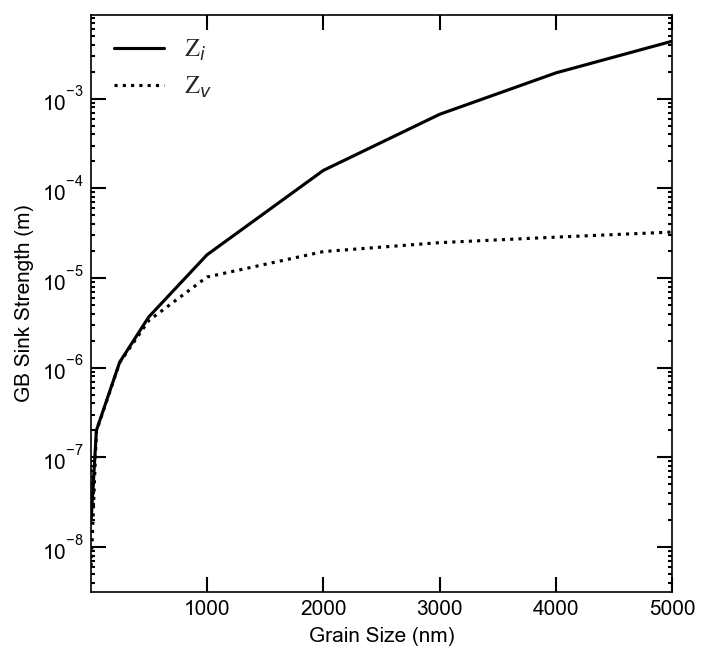
\includegraphics[scale=0.55]{Fig9_a}
        b)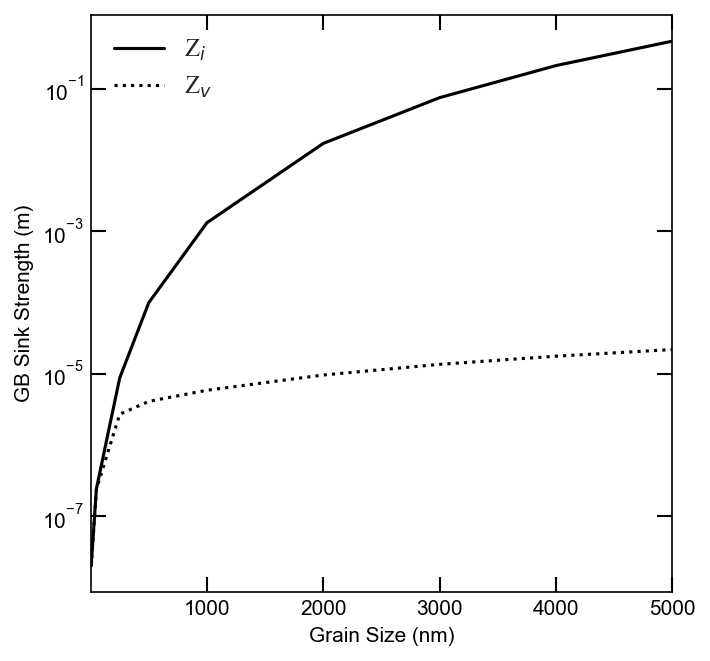
\includegraphics[scale=0.55]{Fig9_b}
        \qquad
        c)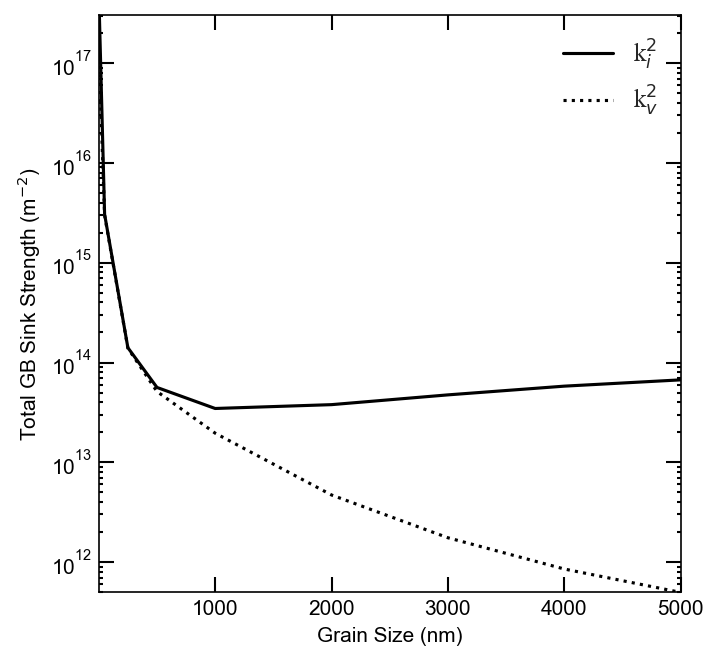
\includegraphics[scale=0.55]{Fig9_c}
        d)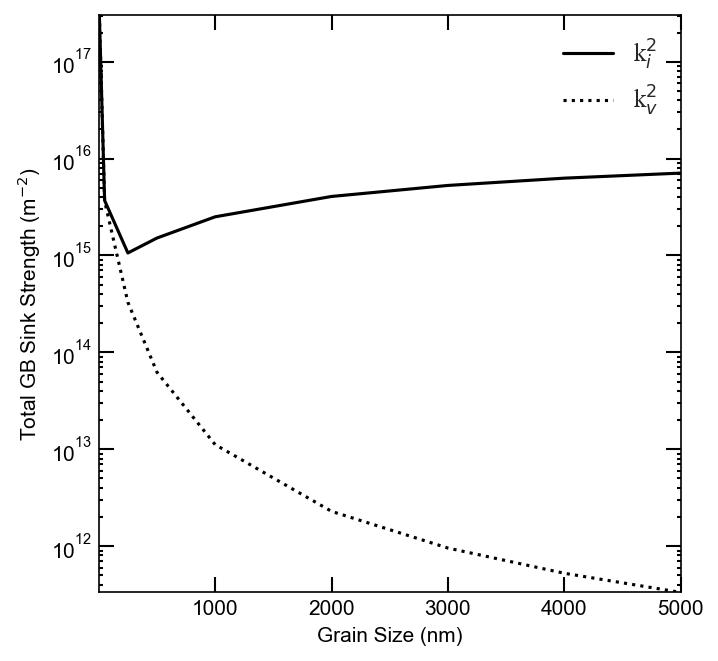
\includegraphics[scale=0.55]{Fig9_d}
        \caption{Change of grain boundary sink strengths with grain size for 5\% production bias. Grain boundary sink strengths, $Z_{gb,i}$ and $Z_{gb,v}$, for a)low dose rate (1e-6 $dpa/s$) and b) high dose rate (1e-3 $dpa/s$). Total grain boundary sink strengths, $k_{gb,i}^2$ and $k_{gb,v}^2$, for c)low dose rate(1e-6 $dpa/s$) and d) high dose rate (1e-3 $dpa/s$). Because of the size- and dose rate-dependent instability, the individual and total boundary sink strengths for interstitials are higher than vacancies above the critical size. This indicates that the boundary changes from neutral to biased at the critical size.}
        \label{figure:sink_strengths_neutron_5_1e-6}
    \end{figure}
    
    \begin{figure}[h!]  %GB Sink Strength - Neutron 1e-6 dpa/s
        \centering
        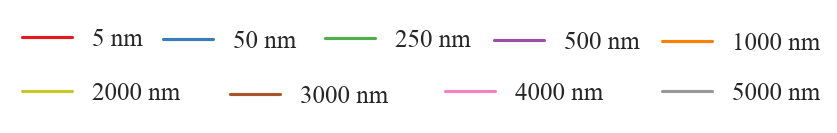
\includegraphics[scale=0.3]{Fig_legend}\\
        a)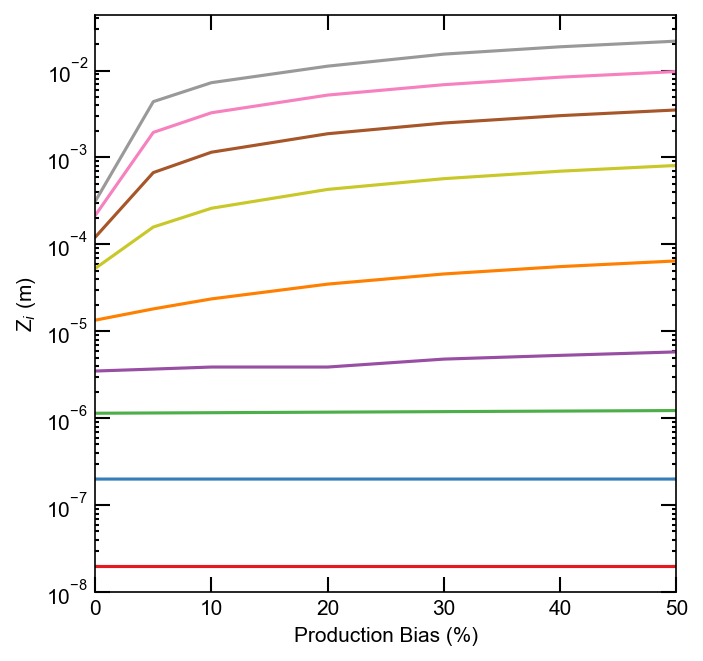
\includegraphics[scale=0.5]{Fig10_a}
        b)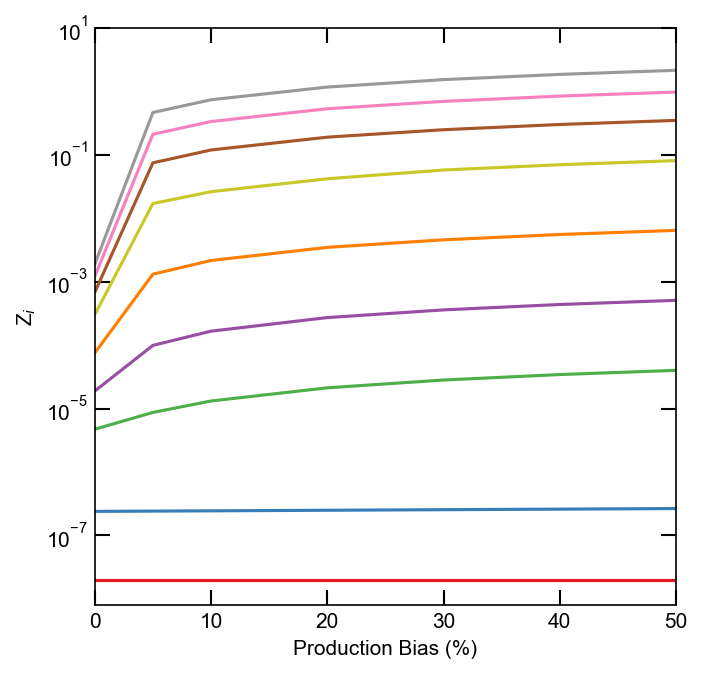
\includegraphics[scale=0.5]{Fig10_b}
        % \includegraphics[scale=0.35]{legend}
        c)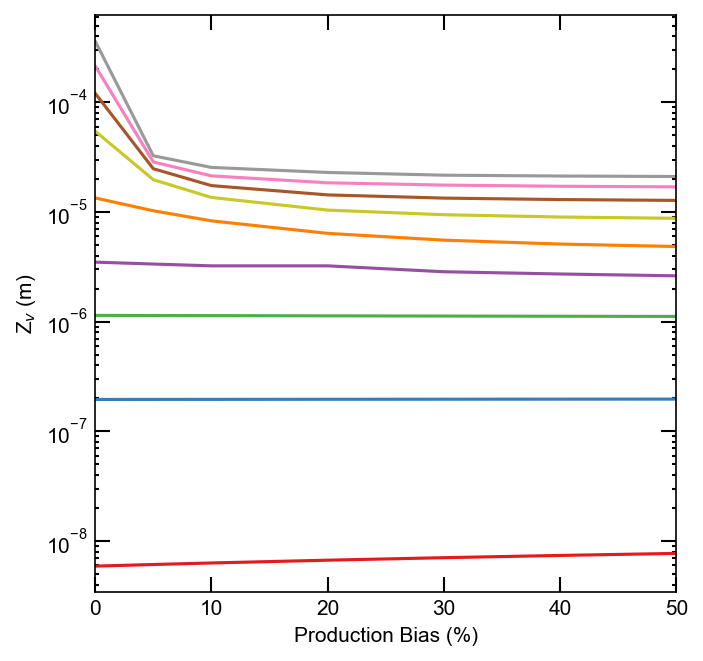
\includegraphics[scale=0.5]{Fig10_c}
        d)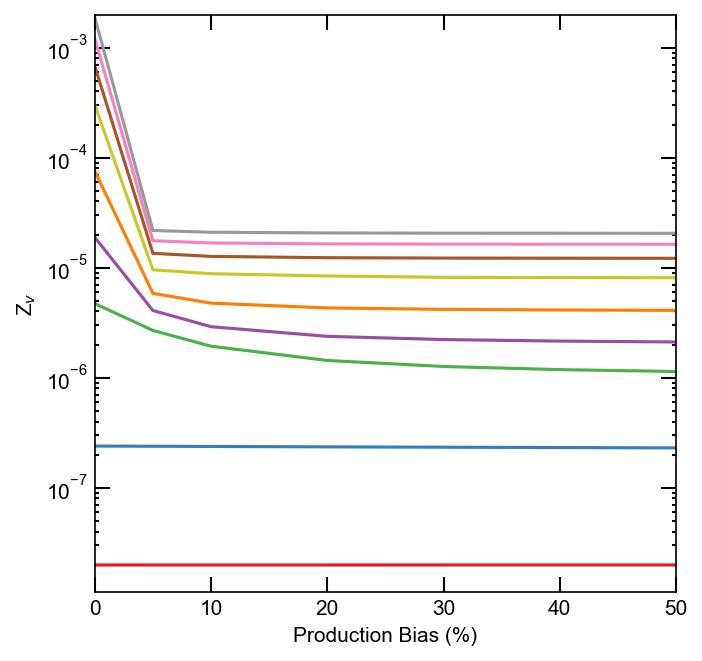
\includegraphics[scale=0.5]{Fig10_d}
        % \includegraphics[scale=0.35]{legend}
        \caption{Change of grain boundary sink strengths with production bias and grain size, a) $Z_{gb,i}$ for low dose rate(1e-6 $dpa/s$), b) $Z_{gb,i}$ for high dose rate(1e-3 $dpa/s$), c) $Z_{gb,v}$ for low dose rate(1e-6 $dpa/s$), d) $Z_{gb,v}$ for high dose rate (1e-3 $dpa/s$). Below the critical size, the boundary sink strengths for both defects are equal and constant (independent of the value of production bias). However, at and above the critical size, the boundary sink strength for interstitials increases with bias, while it decreases with bias for vacancies.}
        \label{figure:sink_strengths_neutron_bias_Z}
    \end{figure}
    
    \begin{figure}[h!]  %GB Sink Strength - Neutron 1e-6 dpa/s
    \centering
        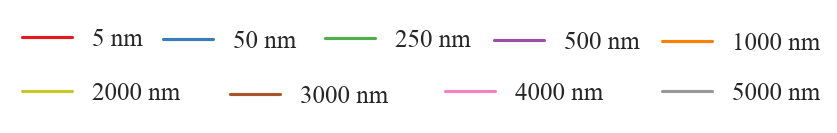
\includegraphics[scale=0.3]{Fig_legend}\\
        a)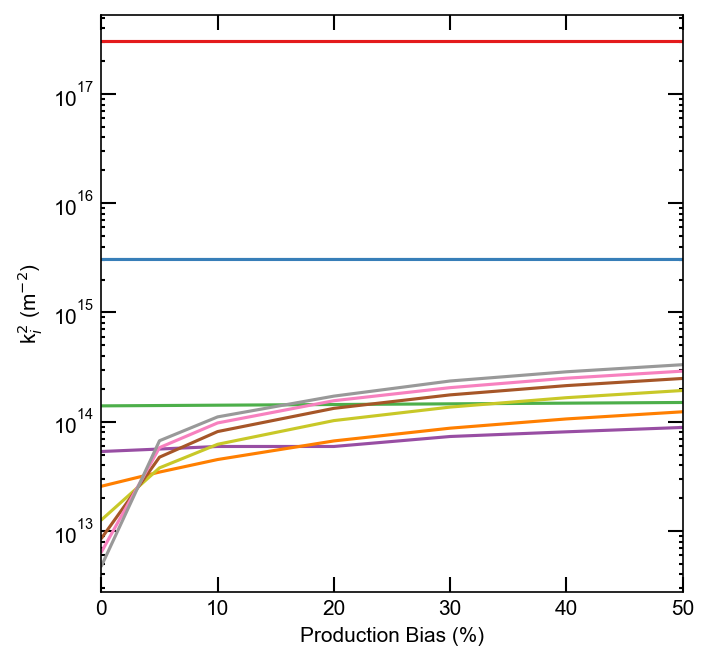
\includegraphics[scale=0.55]{Fig11_a}
        b)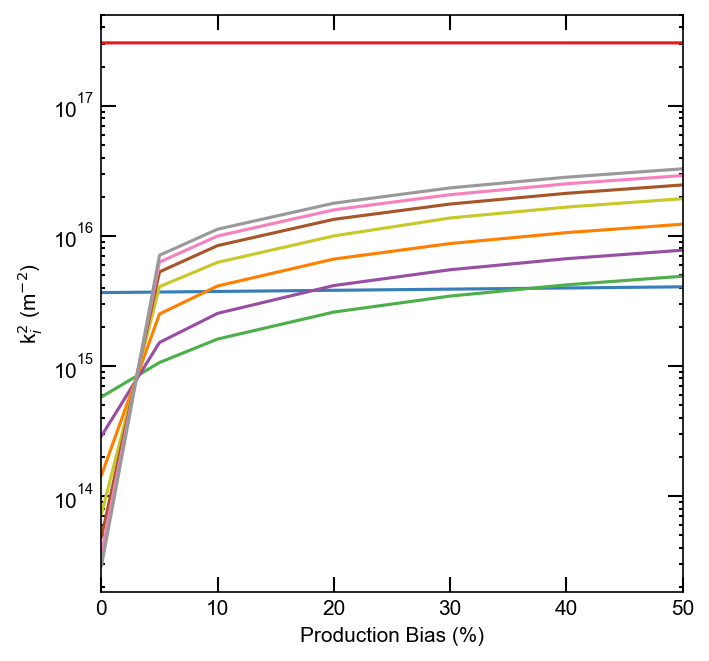
\includegraphics[scale=0.55]{Fig11_b}
        % \includegraphics[scale=0.35]{legend}
        c)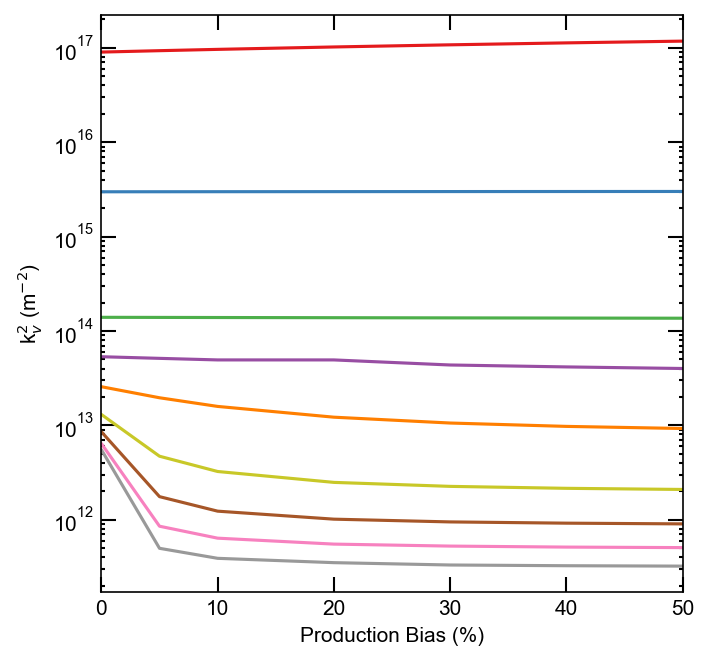
\includegraphics[scale=0.55]{Fig11_c}
        d)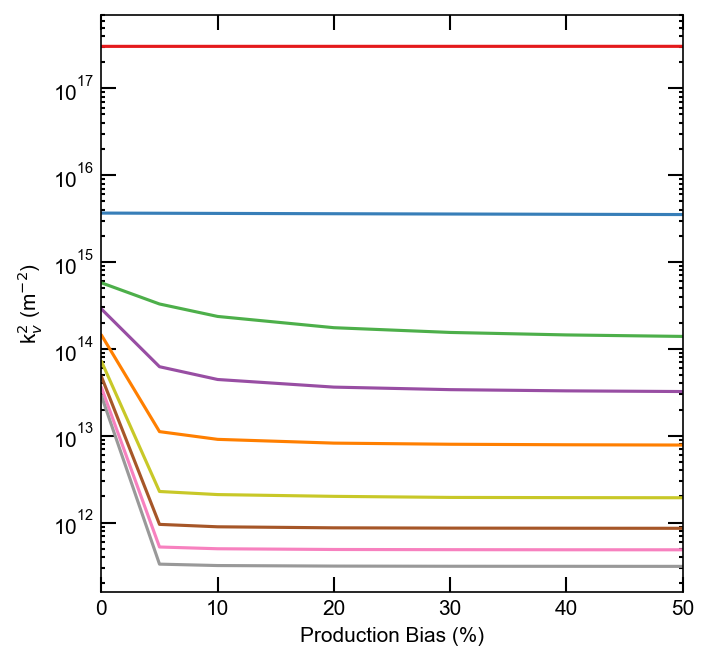
\includegraphics[scale=0.55]{Fig11_d}
        % \includegraphics[scale=0.35]{legend}
        \caption{Change of total grain boundary sink strengths with production bias and grain size, a) $k_{gb,i}^2$ for low dose rate (1e-6 $dpa/s$), b) $k_{gb,v}^2$ for high dose rate (1e-3 $dpa/s$), c) $k_{gb,i}^2$ for low dose rate (1e-6 $dpa/s$), d) $k_{gb,v}^2$ for high dose rate (1e-3 $dpa/s$). The trends for the dependence of the total boundary sinks on production bias are similar to the trends for the individual boundary sink strengths discussed in Fig. \ref{figure:sink_strengths_neutron_bias_Z}.  }
        \label{figure:sink_strengths_neutron_bias_k}
    \end{figure}

\clearpage
    \begin{figure}[h!]  %Sink Strength 3D - Neutron 1e-6 dpa/s
        \centering
        a)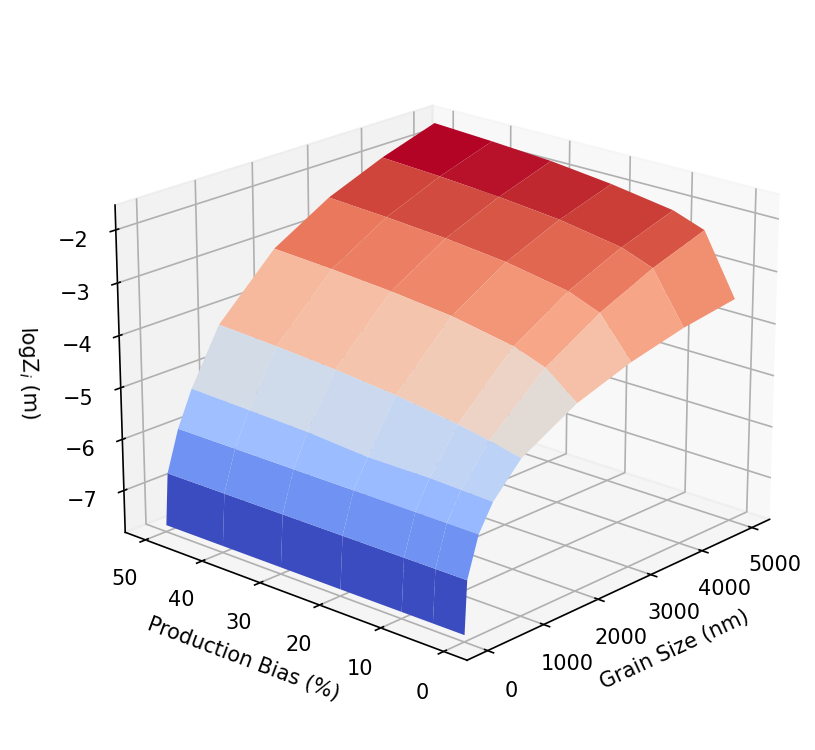
\includegraphics[scale=0.55]{Fig12_a}
        b)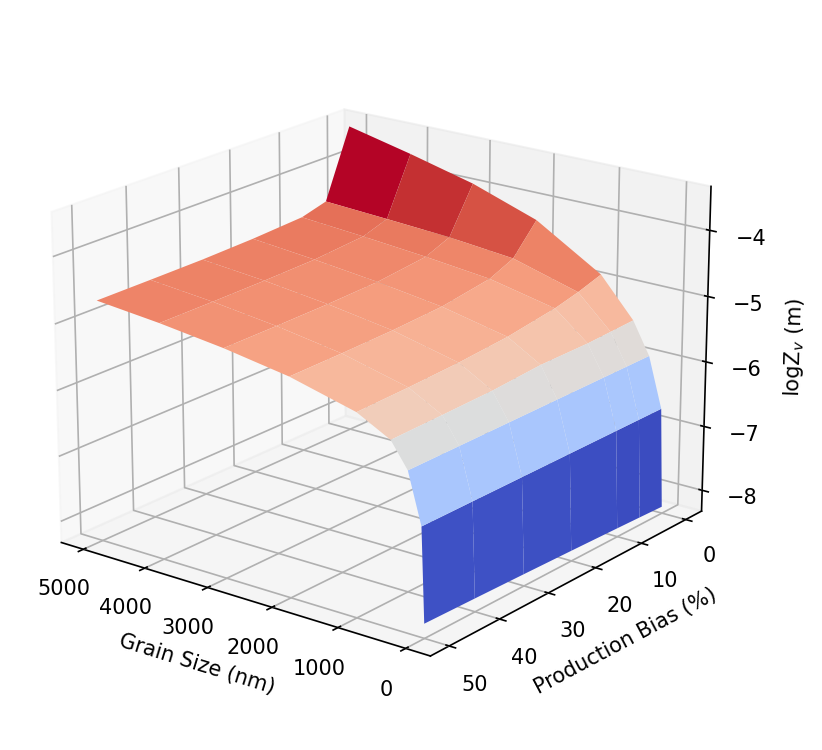
\includegraphics[scale=0.55]{Fig12_b}
        c)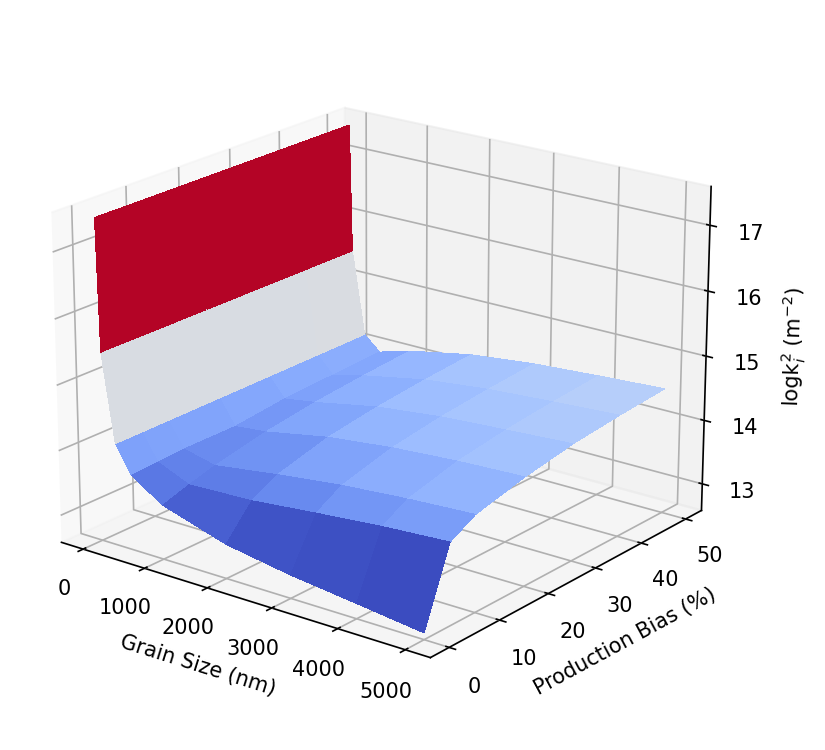
\includegraphics[scale=0.55]{Fig12_c}
        d)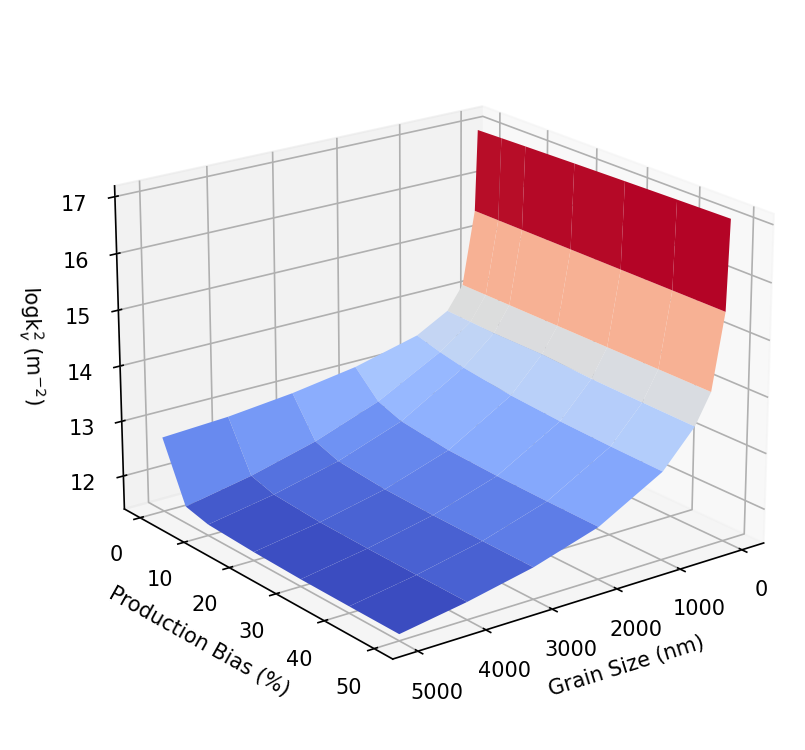
\includegraphics[scale=0.55]{Fig12_d}
        \caption{Change of boundary sink strengths with grain size and production bias for 1e-6 $dpa/s$ dose rate in logarithmic scale: a) interstitial grain boundary sink strength, $Z_{gb,i}$, b) vacancy grain boundary sink strength, $Z_{gb,v}$, c) total interstitial grain boundary sink strength, $k_{gb,i}^2$, d) total vacancy grain boundary sink strength, $k_{gb,v}^2$.}
        \label{figure:sink_strength_moose_neutron_3D}
     \end{figure}

\clearpage
\subsection{Size effect on radiation-induced segregation in Ni-Cr }

The size-dependent instability reported here is expected to render irradiation damage more severe as was discussed in the last section. It was demonstrated that the vacancy supersaturation rises sharply above the critical size (recall Fig. \ref{figure:center_vacancy_supersaturation_neutron}). This will in turn facilitate the clustering of vacancies into voids and/or vacancy loops. The clustering process, though, is highly influenced by material properties such as binding energies of point defects, surface energy, and stacking fault energies. However, a more direct effect for the increase of point defect concentrations and gradients is the radiation induced segregation (RIS) of solute atoms to surfaces/boundaries \citep{was2017}. Depending on whether solute atoms exchange preferably with vacancies or interstitials, they will be depleted or enriched at the surface/boundary, respectively.

Here, we investigate the size effect on the RIS in a Ni-Cr binary alloy. Ni-Cr based alloys are one of the most important materials for current and future advanced nuclear reactors. These alloys show high strength, high resistance to swelling at high temperatures, and superior corrosion performance. Nonetheless, despite their many advantages, radiation induced segregation in these alloys is known to significantly alter their properties \citep{allen_effect_1997,was_emulation_2002,allen_thermal_2007,wharry_systematic_2013}. Therefore, studying the process of RIS in Ni-Cr based alloys is crucial for advancing the utilization of these alloys and improving the safety and performance of reactors.
To investigate radiation-induced segregation in alloys, the inverse Kirkendall model is usually employed \citep{allen_modeling_1998,wharry_mechanism_2014,was2017}. In that model,in addition to the same balance laws of point defects solved above, the continuity equations for the atomic species are coupled and solved concurrently. Specifically, for a binary Ni-Cr system, one has \citep{barr_grain_2015}

\begin{equation}
    \begin{aligned}
    &\frac{\partial C_i}{\partial t} = - \nabla\cdot J_i + K_0 - K_{iv}C_iC_v - K_{is}C_iC_s\\
    &\frac{\partial C_v}{\partial t} = - \nabla\cdot J_v + K_0 - K_{iv}C_iC_v - K_{vs}C_iC_s\\
    &\frac{\partial C_{Cr}}{\partial t} = - \nabla\cdot J_{Cr} \\
    \end{aligned}
    \label{equation:RIS_equations}
\end{equation}

The time derivatives in Eq. \ref{equation:RIS_equations} represent the evolution of the concentration of interstitials ${C_i}$,  concentration of vacancies ${C_v}$,  and concentration of Cr atoms ${C_{Cr}}$. On the right-hand side, first terms ${\nabla\cdot J_i}$ , ${\nabla\cdot J_v}$ and ${\nabla\cdot J_{Cr}}$ are the divergences of the interstitial, vacancy and Cr atoms fluxes. The second term in Eq. \ref{equation:RIS_equations} is a source term representing defect generation with rate constant of $K_0$. Third term ${K_{iv}C_iC_v}$ is a reaction term, referring to the recombination between interstitials and vacancies. The last term is also a reaction term, representing the reaction between the defect $x$ and the sink $s$ with a rate constant of ${K_{xs}}$. 

The diffusivity of element k (Cr or Ni) for defect x (interstitial or vacancy), \textit{$d_{x,k}$} , is defined by the following equation:
\begin{equation}
    \begin{aligned}
    &d_{x,k} = {d_0}^{x,k}\exp(\frac{-{E_m}^{x,k}}{kT})\\
    \end{aligned}
    \label{equation:RIS_diffusivity}
\end{equation}
where ${d_0}^{x,k}$ is pre-exponential factor of Ni or Cr for vacancy or interstitial, ${{E_m}^{x,k}}$ is the migration energy of Ni or Cr for the vacancy or interstitial, $T$ is temperature and $k$ is the Boltzmann constant.

We expressed the partial diffusion coefficient by $D = dN$, where $N$ is atomic fraction and $d$ is diffusivity (see Eq. \ref{equation:RIS_diffusivity}). The spatial dependence resides in the $N$. In contrast, the $d$ is composition independent and contains the kinetic and diffusion information \citep{wiedersich_theory_1979}.

\begin{equation}\begin{aligned}
        &D_{i}^{Cr} = d_{i,Cr}N_{Cr}\\
        &D_{i}^{Ni} = d_{i,Ni}N_{Ni}\\
        &D_{v}^{Cr} = d_{v,Cr}N_{Cr}\\
        &D_{v}^{Ni} = d_{v,Ni}N_{Ni}\\
        &D_{Cr}^{v} = d_{v,Cr}N_{v}\\
        &D_{Cr}^{i} = d_{i,Cr}N_{i}
        \label{equation:RIS_partial}
        \end{aligned}
     \end{equation}
where $D_{i}^{Cr}$ and $D_{i}^{Ni}$ are the partial diffusion coefficients for interstitials via Cr and Ni atoms,  $D_{v}^{Cr}$ and $D_{v}^{Ni}$ are the partial diffusion coefficients for vacancies via Cr and Ni atoms, $D_{Cr}^{v}$ and $D_{Cr}^{i}$ are the partial diffusion coefficients for Cr atoms via vacancies and interstitials. 

The total diffusion coefficients for the vacancies, interstitials and Cr atoms are given as $D_{v}$, $D_{i}$ and $D_{Cr}$, respectively.
\begin{equation}
    \begin{aligned}
    &D_{v} = d_{v,Cr}N_{Cr}+d_{v,Ni}N_{Ni}\\
    &D_{i} = d_{i,Cr}N_{Cr}+d_{i,Ni}N_{Ni}\\
    &D_{Cr} = d_{v,Cr}N_{v}+d_{i,Cr}N_{i}\\
    \end{aligned}
    \label{equation:RIS_totaldiffusioncoefficients}
 \end{equation}   
where $d_{v,Cr}$ and $d_{i,Cr}$ are the vacancy and interstitial diffusivities for Cr, $d_{v,Ni}$ and $d_{i,Ni}$ are the vacancy and interstitial diffusivities for Ni. 

Therefore, fluxes take on the following expressions,
 
 \begin{equation}
    \begin{aligned}
    &J_{v} = d_{v,Cr}\Omega C_{v}\nabla C_{Cr} + d_{v,Ni}\Omega C_{v}\nabla C_{Ni} - D_{v}\nabla C_{v}\\
    &J_{i} = -d_{i,Cr}\Omega C_{i}\nabla C_{Cr} + d_{i,Ni}\Omega C_{i}\nabla C_{Ni} - D_{i}\nabla C_{i}\\
    &J_{Cr} = -D_{Cr}\nabla C_{Cr} + d_{v,Cr}\Omega C_{Cr}\nabla C_{v} - d_{i,Cr}\Omega C_{Cr}\nabla C_{i}\\
    \end{aligned}
    \label{equation:RIS_flux_equations}
 \end{equation}
where $J_{v}$ and $J_{i}$ are the fluxes of vacancies and interstitials, $J_{Cr}$ is flux of the Cr atoms. $\Omega$ is atomic volume.

In this study, a Ni–5Cr binary alloy system was used as model alloy. Ni and Cr properties used in the radiation induced segregation model: lattice parameter is 0.352 $nm$, pre-exponential factor for Ni interstitial diffusivity 5.04e-8 $m^2/s$, pre-exponential factor for Cr interstitial diffusivity 3.20e-7 $m^2/s$, pre-exponential factor for Ni vacancy diffusivity 1.85e-4 $m^2/s$, pre-exponential factor for Cr vacancy diffusivity 2.26e-4 $m^2/s$, activation energy for Ni interstitial diffusivity 0.30 $eV$, activation energy for Cr interstitial diffusivity 0.37 $eV$, activation energy for Ni vacancy diffusivity 1.16 $eV$, activation energy for Cr vacancy diffusivity 1.10 $eV$, vacancy formation energy 1.79 $eV$, interstitial formation energy 4.0 $eV$ \citep{barr_grain_2015}. For all simulations in this section, the Cartesian coordinate system was used to represent planar geometry.

We simulated radiation induced segregation model at an irradiation temperature of 773 $K$, the most common temperature used for RIS studies \citep{allen_thermal_2007,wharry_systematic_2013,barnard_ab_2014,barr_grain_2015} and dose rates of 7e-6 and 1e-3 $dpa/s$. In one of simulations, temperature was varied between 473 $K$ and 1073 $K$ to study its effect. Vacancy and interstitial concentrations were determined as the concentrations at thermal equilibrium for the initial conditions of system. Ni and Cr concentrations are taken as the nominal value in the alloy composition. We assumed that the alloy atoms are randomly distributed throughout the grain at the initial time and bulk sinks are uniformly distributed with a concentration of 1e18 $m^{-3}$. We conducted several simulations to investigate the effects of size, production bias, dose rate, and temperature on RIS in Ni-5Cr. In all of these simulations, the boundary is assumed neutral and perfect, and zero flux boundary condition was used for Cr. Because of the problem symmetry, only one boundary (at x = 0 in the figures) is considered while at the other far end (representing the grain center), zero flux boundary conditions are considered for point defects and Cr. The equations were solved numerically with the initial and boundary conditions, and one-dimension calculations were performed.

Our model predictions for the case of large grains and without bias agree well with the numerical results and experimental data presented in \citep{barr_grain_2015}. However, we demonstrate here a strong dependence of RIS on size and bias, which was not explored in \citep{barr_grain_2015}. The quantitative effects of size and production bias on RIS in Ni-5Cr are presented in Figs. \ref{figure:RIS_773K_0vs5vs10vs20} and \ref{figure:RIS_Cr_50_125_250_500nm_773K}. In Fig. \ref{figure:RIS_773K_0vs5vs10vs20}, the effect of production bias is shown for two different grain sizes at a temperature of 773 $K$ and a dose rate of 1e-3 $dpa/s$. As evident from the figure, the depletion of Cr at the boundary becomes more pronounced as the production bias increases. Both the boundary Cr concentration is reduced, and the depletion layer is widened with bias. This is consistent with the fact that Cr exchanges preferably with vacancies, which rise with bias. However, it is noteworthy that the effect of bias is more apparent in the large grain. For the 500 $nm$ grain with 10\% production bias, the steady-state vacancy concentration is one order of magnitude higher than its corresponding value in the absence of bias. Conversely, the steady-state interstitial concentration is one order of magnitude lower than its corresponding value in the absence of bias. This is because of the size-dependent instability discussed before, i.e., the instability is only triggered in the large grain. In Fig. \ref{figure:RIS_Cr_50_125_250_500nm_773K}, the effect of size on RIS in Ni-5Cr is explicitly investigated for two different dose rates in the presence and absence of bias. Consistent with the results from section 3.1, the size effect saturates above 250 $nm$ in the absence of bias. Nonetheless, in the presence of bias, the depletion of Cr increases with size. Moreover, the rate of increase rises with size. It is also clear that the magnitude of depletion and its size dependence are amplified at higher dose rates. At the low dose rate of 7e-6 $dpa/s$, the model predictions lie within the results obtained before \citep{barr_grain_2015}, where Cr concentration at the boundary reported to be between 2-4\%. Nonetheless, the predictions here for 20\% bias show inverse dependence on grain size, i.e., Cr concentration at the boundary becomes smaller with increasing size. Moreover, at the high dose rate of 1e-3 $dpa/s$, the Cr boundary concentration becomes negligibly small at sizes above 250 $nm$. However, in this case, the treatment of the boundary as a perfect sink is probably no longer valid. 

Lastly, the effect of temperature on RIS in Ni-5Cr was investigated. Fig. \ref{figure:RIS_473vs773vs1073} summarizes the results of simulations conducted for a 500 $nm$ grain irradiated at 1e-3 $dpa/s$ with two different production biases. First, the dependence of point defects on temperature is obvious, i.e., as temperature increases, the steady-state concentration of vacancies decreases, while the interstitial counterpart rises. Therefore, the difference between the point defect concentrations is reduced at high temperature. Moreover, at the highest temperature of 1073 $K$,  
the instability is absent (see Fig. \ref{figure:RIS_473vs773vs1073}a). However, it could still happen at this temperature for higher dose rate, higher production bias, or larger size. Hence, RIS is least observed at the highest temperature. As the temperature decreases, RIS becomes more apparent with higher segregation of Ni and depletion of Cr at the boundary as the production bias increases. RIS is predicted here to be maximum at the lowest temperature of 473 $K$, while it is often reported to be maximum at intermediate temperature \citep{barnard_ab_2014,barr_grain_2015}. This could be attributed to the uncertainties associated with interstitial diffusivities at lower temperature and the validity of the perfect sink assumption, as was discussed in \citep{barnard_ab_2014}. Nevertheless, the combined effect of size and production bias on RIS is clear.

     \begin{figure}[h!]  %
        \centering
        a)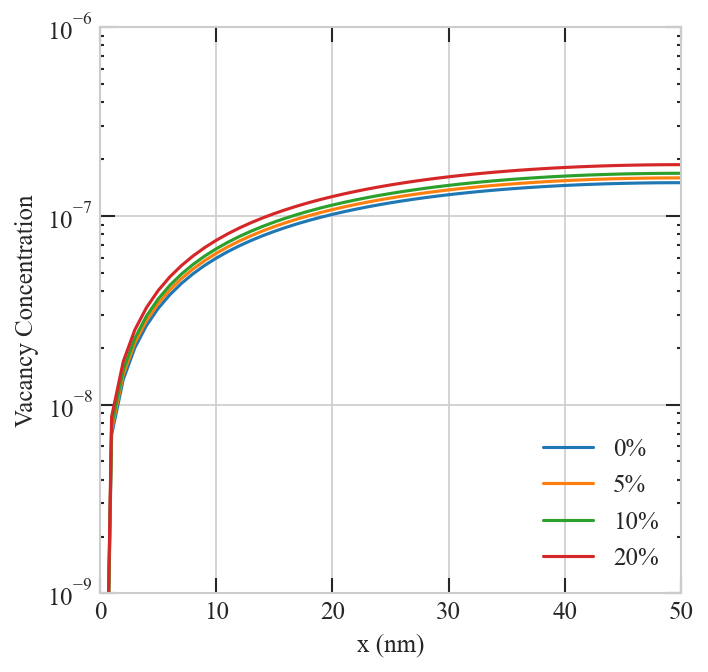
\includegraphics[scale=0.55]{srrt/plots/Fig13_a.png}
        b)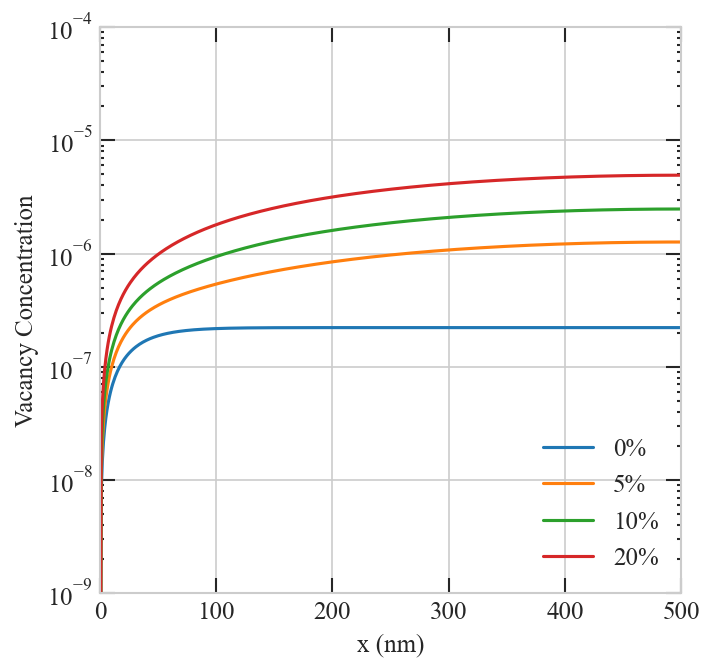
\includegraphics[scale=0.55]{srrt/plots/Fig13_b.png}
        \\
        c)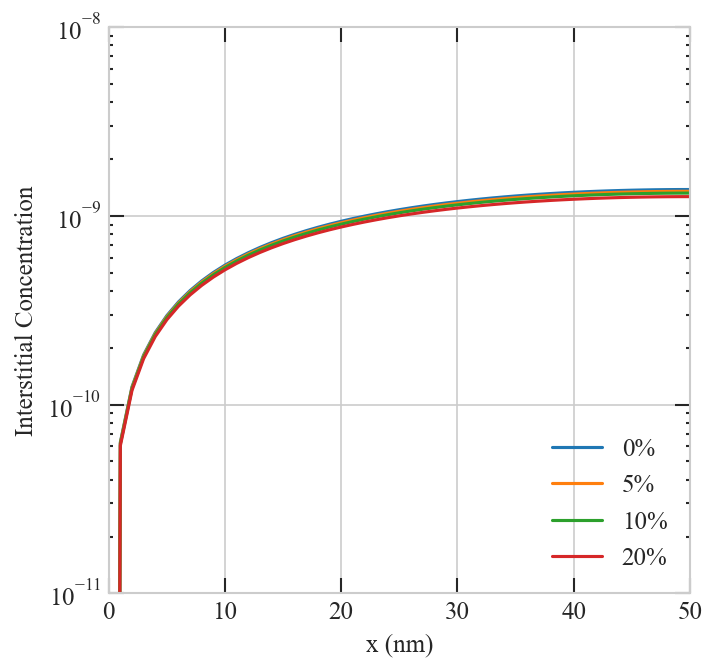
\includegraphics[scale=0.55]{srrt/plots/Fig13_c.png}
        d)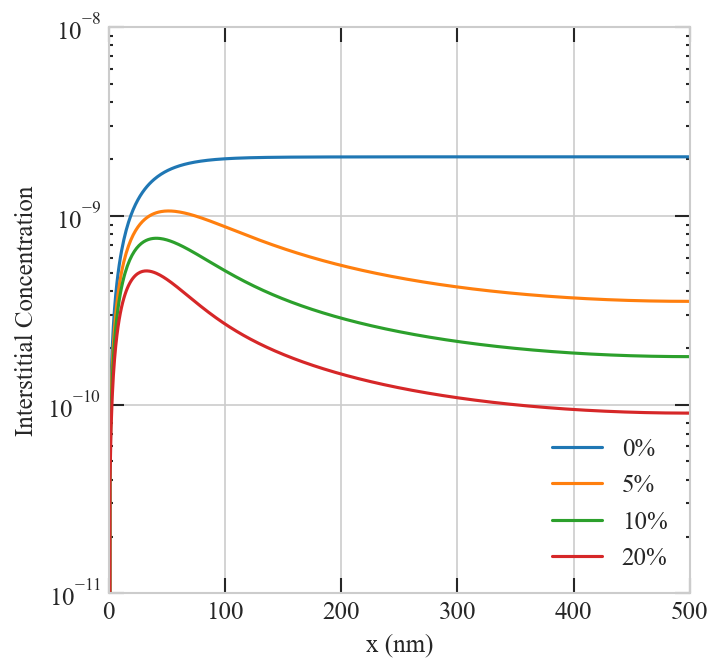
\includegraphics[scale=0.55]{srrt/plots/Fig13_d.png}
        \\
        e)\includegraphics[scale=0.55]{srrt/plots/Fig13_e.png}
        f)\includegraphics[scale=0.55]{srrt/plots/Fig13_f.png}
        \caption{Effect of production bias on the steady-state concentration profiles of point defects in Ni-Cr at 1e-3 $dpa/s$ . Upper row: vacancy concentration for a) 50 $nm$ and b) 500 $nm$ grains. Middle row: interstitial concentration c) 50 $nm$ and d) 500 $nm$ grains. Lower row: chromium concentration e) 50 $nm$ and f) 500 $nm$ grains. The effect of production bias is more apparent at larger sizes because of the size-dependent instability discussed in section 3.1}
        \label{figure:RIS_773K_0vs5vs10vs20}
      \end{figure}

\clearpage  
    \begin{figure}[h!]  %
        \centering
        a)\includegraphics[scale=0.55]{srrt/plots/Fig14_a.png}
        b)\includegraphics[scale=0.55]{srrt/plots/Fig14_b.png}
        c)\includegraphics[scale=0.55]{srrt/plots/Fig14_c.png}
        d)\includegraphics[scale=0.55]{srrt/plots/Fig14_d.png}
        \caption{Effect of grain size on the steady-state concentration profiles of Chromium. Upper row: concentration profiles of Chromium at 1e-3 $dpa/s$  and a) 0\% and b) 20\% production bias. Lower row: concentration profiles of Chromium at 7e-6 $dpa/s$  and c) 0\% and d) 20\% production bias. Similar to the case of pure Ni (recall Fig. \ref{figure:concentrations_neutron_5}), size effect saturates above $\approx$125-250 $nm$ (depending on dose rate) in the absence of bias, while it continues to become stronger in the presence of bias. The depletion of Cr increases with bias and size. This increase is more pronounced at higher dose rates.}
        \label{figure:RIS_Cr_50_125_250_500nm_773K}
        %(recall Figs. \ref{figure:concentrations_micro_nano_neutron_5_1e-3} and \ref{figure:concentrations_neutron_5})
    \end{figure}
   

    \begin{figure}[h!]  %
        \centering
        a)\includegraphics[scale=0.55]{srrt/plots/Fig15_a.png}
        b)\includegraphics[scale=0.55]{srrt/plots/Fig15_b.png}
        c)\includegraphics[scale=0.55]{srrt/plots/Fig15_c.png}
        d)\includegraphics[scale=0.55]{srrt/plots/Fig15_d.png}
        e)\includegraphics[scale=0.55]{srrt/plots/Fig15_e.png}
        f)\includegraphics[scale=0.55]{srrt/plots/Fig15_f.png}
        \caption{The effect of temperature on the steady-state concentration profiles of defects and atoms in a 500 $nm$ Ni-Cr grain at 1e-3 $dpa/s$ for 5\% and 20\% biases: a) interstitial, b) vacancy, c) chromium, d) nickel, e) chromium 250 $nm$ close-up, and f) nickel 250 $nm$ close-up.}
        \label{figure:RIS_473vs773vs1073}
    \end{figure}

\clearpage
\section{Conclusions}

In this work, we conducted a detailed study of the effects of surface and size on the transient and steady-state behavior of point defects in irradiated solids. Pure Ni and Ni-Cr were utilized as model systems. The balance equations for point defects were solved simultaneously using a fully-coupled and fully-implicit scheme implemented in the MOOSE framework.    

It was found that, in the presence of production bias, the effects of surface and size are pronounced even at low the surface to volume ratio. This was attributed to a surface-induced and size-regulated instability. This instability appears above a critical size between 100-500 $nm$. The critical size decreases with increasing dose rate and/or production bias or lowering the temperature. Our detailed analysis revealed that this instability is triggered due to the fact that production bias breaks the symmetry of point defects flow to the surface/boundary, effectively transforming it into a biased sink. Below the critical temperature and at the threshold size, the imbalance in the flow of point defects is enough to create a pattern that favors the separation of vacancies and interstitials. Once this pattern develops, anomalies in the dependence on size for the steady-state concentrations of point defects and the surface/boundary sink strength are observed. Specifically, it is shown that once this instability is initiated, while the steady-state vacancy concentration continues to increase with size, its interstitial counterpart starts to decrease with size. On the other hand, while the surface/boundary sink strength for vacancies continue to decrease with size, its interstitials counterpart starts to increase with size. Hence, the developed instability and the resultant patterns will promote irradiation effects in materials. Indeed, this was demonstrated here by investigating vacancy supersaturation in Pure Ni and radiation-induced segregation in Ni-Cr. In the former, it was shown that vacancy supersaturation in Ni increases with size and the rate of increase also rises with size. In the latter, it was shown that the magnitude of enrichment/depletion of Ni/Cr at the boundary increases with size and the width of the enrichment/depletion layer also increases with size.

It is worth noting that the above-mentioned instability and the resultant pattern and anomalies are absent in nanomaterials (with sizes $<$ 100 $nm$). This gives a new perspective on the resistance of these materials to irradiation as opposed to the susceptibility of conventional materials (with sizes $>$ 100 $nm$) to irradiation. In conventional materials, the developed pattern of point defects facilitates the clustering and formation of extended defects. Conversely, the exact opposite is observed in nanomaterials.

The results obtained here agree well with experimental observations in irradiated materials. For instance, the patterns appearing in the steady-state concentration profiles of point defects and the resultant pattern in the vacancy supersaturation agree well with the well-known observation of the development of void denuded zones in the vicinity of grain boundaries in irradiated polycrystalline solids \citep{was2017}. Notably, our model can capture this behavior without the added assumption of 1D migration of interstitials, which was previously thought as a necessary condition to explain void swelling and its heterogeneity near the interfaces in materials. Moreover, the dependence of irradiation tolerance in materials on size and temperature demonstrated here is in agreement with the comprehensive experimental study conducted by \citep{mao2019} on irradiated Cu and Cu-W alloys.

It is also noteworthy to point that models/simulations that ignore defects diffusion to localized sinks (e.g., surfaces/boundaries), bulk recombination of point defects, or production bias are incapable of capturing this size-dependent effects. Such reduced-ordered models or lower-fidelity simulations will not only have inaccurate quantitative predictions but may also have completely wrong qualitative predictions. Therefore, precautions must be taken in developing/conducting such models/simulations and interpreting their results.

It is also important to discuss the limitations of the current study. First, the treatment of the production bias here is simplified, i.e., its value was considered as unknown, and a parametric study of its effect was conducted. However, exact values for different irradiation types and conditions can be obtained through a multiscale modeling approach that simulate the development of irradiation cascades and the clustering of point defects \citep{was2017}. Second, the evolution of extended defects and their heterogeneity were ignored. The co-evolution of point and extended defects must be accounted for to develop a comprehensive understanding of irradiation effects in materials. Third, further microstructure descriptors in addition to size should be incorporated into the model since grain morphology, interfacial energy, and misorientation are expected to play important roles in the response of grain boundaries to irradiation \citep{was2017}. Alleviating these limitations will be the focus of upcoming studies.

Lastly, we want to reflect on the implications of this study on the on-going debate on the utilization of ion irradiation to mimic neutron irradiation to accelerate the qualification of novel materials for advanced reactors. It is clear form all the results presented here that there is a strong and non-linear quantitative dependence, regardless of size, on production bias, dose rate, and temperature, i.e., irradiation type and conditions. Moreover, when surface and size effects are considered, qualitative differences in the irradiation response of materials to different irradiation types are expected. In fact, we proved that, in addition to its known dependence on material and size/microstructure, the surface/boundary sink strength is dependent on irradiation type. Hence, the generalization of predictions based on ion irradiation data to neutron irradiation is generally inaccurate. However, the utilization of physics-based models and high-fidelity simulations, as presented here, can be used to bridge the gap between the different irradiation types and improves the generalization. This can be accomplished by leveraging ion irradiation data to validate the models and then using the models to simulate the response under neutron irradiation.
         

\section*{Acknowledgements}
 
The authors would like to acknowledge the support from a start-up grant from Texas A\&M University. Portions of this research were conducted with the advanced computing resources provided by Texas A\&M High Performance Research Computing.         

\section*{Code and data availability}

MOOSE is an open source code that can be freely downloaded from \href{https://mooseframework.inl.gov/}{https://mooseframework.inl.gov/}. The input files and plots for this study are available for download from a public repository located at
\href{https://github.com/abdurrahmanozturk/SRRT}{https://github.com/abdurrahmanozturk/SRRT}. All data generated during this study can be reconstructed by running MOOSE input files.
\clearpage
\bibliographystyle{frontiersinSCNS_ENG_HUMS} % for Science, Engineering and Humanities and Social Sciences articles, for Humanities and Social Sciences articles please include page numbers in the in-text citations
%\bibliographystyle{frontiersinHLTH&FPHY} % for Health, Physics and Mathematics articles
\bibliography{references}

%%% Make sure to upload the bib file along with the tex file and PDF
%%% Please see the test.bib file for some examples of references

\end{document}